\documentclass[10pt]{article}
\usepackage[margin=0.75in]{geometry}
\usepackage[fontsize=9.5pt]{fontsize}
\linespread{0.97}
\renewcommand{\topfraction}{0.95}
\renewcommand{\bottomfraction}{0.9}
\renewcommand{\textfraction}{0.05}
\renewcommand{\floatpagefraction}{0.85}
\setcounter{topnumber}{3}
\setcounter{totalnumber}{5}
\setlength{\textfloatsep}{10pt plus 2pt minus 2pt}
\setlength{\intextsep}{8pt plus 2pt minus 2pt}
\usepackage{amsmath,amssymb}
\usepackage{booktabs}
\usepackage{graphicx}
\usepackage{caption}
\usepackage{subcaption}
\usepackage[numbers,sort&compress]{natbib}
\usepackage{microtype}
\usepackage{xcolor}
\usepackage{array}
\usepackage{multirow}
\usepackage{float}
\usepackage{enumitem}
\usepackage[hidelinks]{hyperref}
\captionsetup{font=small,labelfont=bf,skip=4pt}
\setlength{\abovecaptionskip}{4pt}
\setlist{nosep,leftmargin=*}
\newcommand{\E}{\mathbb{E}}
\newcommand{\pos}[1]{\left[#1\right]_{+}}
\newcommand{\code}[1]{\texttt{#1}}
\newcommand{\PROMOTE}{\textsc{promote}}
\newcommand{\REVERT}{\textsc{revert}}

\title{Priced Runtime Control over Frozen Agent Harnesses:\\
a Learned Orchestrator, an Off-Policy Promotion Gate, and Drift Metrics\\[4pt]
\large Technical report, draft v0.1}
\author{Navid Mehrdad}
\date{October 2026}

\begin{document}
\maketitle

\begin{abstract}
Agent harnesses contain per-request decisions that nobody prices: which model tier answers, whether a sub-result is verified, whether an answer is refined, which specialist is delegated to. The field evolves harnesses at design time; this report studies the complementary runtime problem. We keep the harness frozen and learn a small, cost-priced controller at its decision points, with three pieces: a softmax-linear (or small-LLM) policy trained offline from logged episodes under a budget whose price $\lambda$ is a learned Lagrange multiplier; an off-policy promotion gate that admits a candidate only when doubly-robust (DR) estimates with bootstrap confidence intervals certify quality and cost; and priced backward/forward-transfer metrics for the harness changing under the controller. Six experiments are reported, with negative results stated as results. On a simulator the gate promotes a candidate whose DR interval covers the ground truth, and a gated retrain recovers $+0.033$ of the $-0.045$ that drift costs a frozen controller. On CRMArena-Pro (150 tasks $\times$ 3 tiers, \$59.90) the per-task oracle beats every fixed tier at lower cost, and with three times the data the learned per-category policy beats every fixed tier held-out on quality and cost at once (0.623 at \$0.082 against the frontier tier's 0.616 at \$0.143), while the budgeted controller exceeds frontier quality at 27\% less cost; at 50 tasks the same policies memorised and lost, and the gate said so. On the realised one-arm log the doubly-robust gate promotes on one draw and reverts on another, 10\% of redraws promote, and certifying a \$0.005 budget margin remains a thousand-task matter. A GRPO-trained 1.7B-parameter controller never found the budgeted optimum from near-identical rollout groups; an SFT warm start did the work and GRPO's contribution was the price ($\lambda\approx0.44$). A planner/worker/verifier decomposition scores below a single mid-tier agent (0.480 vs 0.608), its verifier flags 92\% of wrong and 96\% of correct episodes, and an orchestration reward model on process features has out-of-fold AUROC 0.469 against 0.821 for the task category alone. Priced self-refinement after a cheap answer is dominated by buying a better tier up front ($-0.174\pm0.085$ paired at equal cost). The centrepiece is a continual orchestrator over a frozen multi-agent structure on a simulator calibrated to the real logs, under four pre-registered harness stages over 40 days: the online learner has the lowest regret of every learned arm (1.26 vs 2.60 frozen and 3.03--3.46 for static routers), recovers after every stage, and has bounded, mostly positive orchestrator-level BWT; but a fixed mode (\code{never\_verify}, regret 0.56; $0.74\pm0.08$ against the learner's $1.06\pm0.21$ over 5 seeds) beats it over the whole stream. That headline is a cold-start artefact: the learner spends 12 days on the uniform exploration policy before its first promotion, crosses the fixed mode around day 22--25 and wins every stage window after that (held-out regret from day 25: 0.22 vs 0.50), and its post-crossover edge at the last stage survives 5 seeds ($+0.031\pm0.007$). A 5-seed verifier ablation shows the fixed mode's win is itself an artefact of the measured verifier and the 8-call cap: with an informative verifier and a cap the retries do not consume, verification helps ($+0.029\pm0.001$ quality for $+18\%$ cost) and \code{always\_verify} becomes the right fixed mode. The gate reverts 32 of 40 candidates (23 false alarms on the quality criterion), and the AWR variant is promoted 14 times on a DR estimate biased by $+0.68$. The pattern across all six: the signal, not the learner, is the bottleneck.
\end{abstract}

\section{Introduction}

An agent harness is the scaffold around a model: the loop that decides which tool runs next, which model answers, whether a step is checked, when the episode ends. Inside that loop sit decisions that are made per request, in microseconds, by a rule somebody wrote: ``always use the large model'', ``verify every sub-result'', ``refine if confidence is low''. Each decision has a price in dollars and latency, and the rule does not see it.

Recent work treats the harness itself as the object of optimisation, at design time. The Darwin G\"odel Machine evolves self-improving agents \citep{dgm2025}; GEPA evolves prompts by reflection \citep{gepa2025}; DarwinX \citep{darwinx2026}, Meta-Harness \citep{metaharness2026}, EnvHarness \citep{envharness2026} and HarnessX \citep{harnessx2026} search over harness designs; EvoHarnessBench \citep{evoharnessbench2026} grows a harness $H_t=\{\text{tools},\text{skills},\text{specialist agents}\}$ monotonically by stages and measures what a \emph{fixed} agent policy forgets or gains per axis, reporting that agent-pool expansion alone gives $-34.7\%$ backward transfer. SkillOrchestra \citep{skillorchestra2026} routes each query to a typed agent in a pool by a learned competence profile with an explicit cost penalty, learned once from traces and then served statically.

This report studies the complementary problem. The harness is frozen; what moves is a small controller at its per-step decision points, trained from logged traffic, priced per request, and put into service only through a statistical gate. Three artefacts make up the method:
\begin{itemize}
\item \textbf{A priced controller.} A policy over $(\text{op},\text{tier})$ pairs whose objective is quality minus a learned price of cost, trained offline by constrained group-relative policy optimisation on replay (or advantage-weighted regression with inverse-propensity weights), with the Lagrange multiplier found by damped dual ascent against a per-task budget and the served policy the iterate average.
\item \textbf{An off-policy promotion gate.} Every served decision logs its propensity, exploration included, so a candidate policy can be scored on logged traffic by IPS, SNIPS and doubly-robust estimators with percentile-bootstrap confidence intervals, and is promoted only when the DR lower quality bound and the DR upper cost bound clear two bars.
\item \textbf{Drift metrics.} Priced backward and forward transfer in the sense of \citet{lopezpaz2017gem}, applied to the priced objective of the controller as the harness is repriced, re-versioned or grown.
\end{itemize}

Six experiments exercise these pieces, in increasing realism: a simulator pipeline (gate, drift, retrain); a counterfactual collection on CRMArena-Pro \citep{crmarenapro2025}; the gate's sample-size behaviour on that log; a 1.7B-parameter LLM as the controller; process-verified multi-agent orchestration; priced Socratic self-refinement; and the centrepiece, a continually trained orchestrator over a frozen multi-agent structure under scripted harness stages. Several results are negative, and they are reported as results: they say where the signal needed by a learned controller is and is not present, which is the question that decides whether a runtime controller earns its place at all. Every number in this report is taken from the committed result files of the public repository; nothing is re-estimated here.

\section{Problem setting}
\label{sec:problem}

\paragraph{The harness as a frozen decision process.}
A harness exposes, at each step $t$ of an episode on task $x$, an observable state $s_t$ and a legal set $\mathcal{A}(s_t)$ of actions $a=(\text{op},\text{tier})$: an operation the harness can run (answer, retrieve, verify, escalate, delegate, re-plan, call a tool, engage a skill) on a model tier (cheap, mid, frontier). The harness's own transition $s_{t+1}\sim P_H(\cdot\mid s_t,a_t)$ is fixed; the controller $\pi(a\mid s)$ only chooses among what is legal. Each step has a realised cost $c_t$ (tokens $\times$ list price) and latency $\ell_t$; a terminal quality $q\in[0,1]$ is the harness's own score. We write $C=\sum_t c_t$ and $L=\sum_t\ell_t$. The harness is a frozen MDP over the controller's decision points, and the controller is the only thing trained.

\paragraph{Priced objective.}
The product specification is a budget, so the objective is
\begin{equation}
J(\pi)=\E_\pi[q]-\lambda\,\E_\pi[C]-\mu\,\E_\pi[L],
\label{eq:J}
\end{equation}
with $\mu=0$ in every experiment here (latency is logged but not priced), and the constrained form
\begin{equation}
\max_\pi\ \E_\pi[q]\quad\text{s.t.}\quad \E_\pi[C]\le B,
\qquad
\mathcal{L}(\pi,\lambda)=\E_\pi[q]-\lambda\big(\E_\pi[C]-B\big),\ \lambda\ge0 .
\label{eq:lagrangian}
\end{equation}
The price $\lambda$ is learned by projected dual ascent on an exponential moving average $\hat c$ of realised episode cost, with a proportional damping term (the PID-Lagrangian of \citet{stooke2020pid} without the derivative term; cf.\ RCPO \citep{tessler2018rcpo}):
\begin{equation}
\hat c_k=\rho\,\hat c_{k-1}+(1-\rho)\,\bar C_k,\qquad
\lambda^{\mathrm{int}}_k=\pos{\lambda^{\mathrm{int}}_{k-1}+\eta\,(\hat c_k-B)},\qquad
\lambda_k=\pos{\lambda^{\mathrm{int}}_k+k_p\,(\hat c_k-B)} .
\label{eq:dual}
\end{equation}
Primal--dual iterates orbit the budget rather than converging to it, so the served policy is the iterate average $\bar\pi(a\mid s)=\frac{1}{|\mathcal{S}|}\sum_{W\in\mathcal{S}}\pi_W(a\mid s)$ over weight snapshots $\mathcal{S}$ from the second half of training \citep{nedic2009saddle}, and $\bar\lambda$ is the mean price over the same half.

\paragraph{Policy class and logged propensities.}
The linear controller is a softmax over soft-clipped logits, mixed with $\epsilon$-exploration:
\begin{equation}
z=L\tanh\!\big(Wx/L\big),\qquad
\pi_\epsilon(a\mid x)=(1-\epsilon)\,\mathrm{softmax}_{\mathcal{A}}(z)_a+\frac{\epsilon}{|\mathcal{A}|},
\label{eq:policy}
\end{equation}
where $x=\phi(s)$ is a feature vector and the softmax is over the legal set. The logit clip keeps the softmax steerable by $\lambda$ and keeps importance ratios bounded. The propensity written to the log is $\mu_t=\pi_\epsilon(a_t\mid x_t)$, exploration included, so every served log is usable for off-policy evaluation (the logging discipline of \citet{bottou2013counterfactual,li2011unbiased}).

\paragraph{Constrained GRPO on replay.}
When the harness can be re-rolled from a logged state (a simulator or a counterfactual lookup table), training samples a logged state $s$, draws a group of $G$ continuations from the policy \emph{as served} ($\pi_\epsilon$, so the cost the dual variable tracks is the served cost), scores each by $R_i=q_i-\lambda C_i$ and uses the group-relative advantage with the group mean as baseline \citep{shao2024grpo}:
\begin{align}
A_i&=R_i-\frac{1}{G}\sum_{j=1}^G R_j,\qquad
\nabla_W\mathcal{L}=\sum_i A_i\sum_t\nabla_W\log\pi_\epsilon(a^i_t\mid x^i_t),
\label{eq:grpo}\\
\nabla\log\pi_\epsilon(a\mid x)&=\frac{(1-\epsilon)\,\pi(a\mid x)}{\pi_\epsilon(a\mid x)}\,\nabla\log\pi(a\mid x).
\label{eq:epsscore}
\end{align}
The last factor is the score correction for the $\epsilon$-mixture: the gradient of the mixed policy is the bare softmax's score scaled by the share of the served probability that the softmax contributes.

\paragraph{Advantage-weighted regression with inverse propensities.}
When no replay exists, the trainer is AWR \citep{peng2019awr} on logged steps with return $R_i=q_i-\lambda\,C^{\to}_i$ (cost-to-go from the step), a per-bucket value baseline $\hat V$, and weights corrected by the logged propensity and self-normalised over the batch:
\begin{equation}
A_i=R_i-\hat V(b(x_i)),\qquad
w_i=\frac{\exp(A_i/\beta)/\mu_i}{\sum_j\exp(A_j/\beta)/\mu_j},\qquad
\max_W\ \sum_i w_i\log\pi(a_i\mid x_i).
\label{eq:awr}
\end{equation}
Here $\lambda$ is a fixed price. Logged counterfactual arms, when present, are added as extra records (offline RL can only reweight what the log contains).

\paragraph{Off-policy estimators.}
For an episode $i$ with per-step rewards $r^i_t$ (the terminal quality, or the per-step cost) and cumulative ratio $\rho^i_{0:t}=\prod_{k\le t}\pi(a^i_k\mid s^i_k)/\mu^i_k$ clipped at $\rho_{\max}=50$,
\begin{align}
\hat V_{\mathrm{IPS}}&=\frac1n\sum_i\sum_t\rho^i_{0:t}\,r^i_t, \qquad
\hat V_{\mathrm{SNIPS}}=\sum_t\frac{\sum_i\rho^i_{0:t}\,r^i_t}{\sum_i\rho^i_{0:t}},
\label{eq:ips}\\
\hat V_{\mathrm{DR}}&=\frac1n\sum_i\Big[\hat V(s^i_0)+\sum_t\rho^i_{0:t}\big(r^i_t+\hat V(s^i_{t+1})-\hat Q(s^i_t,a^i_t)\big)\Big],\qquad
\hat V(s)=\sum_a\pi(a\mid s)\,\hat Q(s,a),
\label{eq:dr}
\end{align}
the per-decision importance-sampling estimator of \citet{precup2000eligibility}, the self-normalised estimator of \citet{swaminathan2015snips}, and the sequential doubly-robust estimator of \citet{jiang2016dr} (see also \citealp{thomas2016magic}). The direct model $\hat Q$ is a per-feature-bucket mean fitted from the log and iterated under the candidate, i.e.\ bucketed fitted-Q evaluation \citep{le2019batch}; the clip biases DR only through the direct-model residual. On a first-step contextual bandit (one decision per task, fixed continuation) the bandit form of \citet{dudik2011dr} applies with a \emph{cross-fitted} direct model:
\begin{equation}
\hat V_{\mathrm{DR}}=\frac1n\sum_i\Big[\sum_a\pi(a\mid x_i)\,\hat Q^{(-i)}(x_i,a)+w_i\big(r_i-\hat Q^{(-i)}(x_i,a_i)\big)\Big],\qquad w_i=\frac{\pi(a_i\mid x_i)}{\mu_i},
\label{eq:drbandit}
\end{equation}
where $\hat Q^{(-i)}$ is fitted leaving out task $i$ (the cross-fitting argument of \citet{chernozhukov2018dml}: an in-sample direct model shares the logged reward it corrects and shrinks the correction toward zero at small $n$). For multi-step orchestration logs with 2--4 decisions over 12 actions, a per-decision variant treats each logged decision as a bandit sample with single-step ratio $w_t=\pi(a_t\mid x_t)/\mu_t$ and reward the episode's quality or cost-to-go; it values changing one decision while the rest of the episode stays as logged, trading bias for ratios bounded by $|\mathcal{A}|/\epsilon$. Every estimate is reported with its effective sample size $\mathrm{ESS}=(\sum_i w_i)^2/\sum_i w_i^2$ \citep{kish1965survey}.

\paragraph{The gate.}
Confidence intervals are percentile bootstraps over episodes (over tasks, with all logged arms of a task together, in the bandit case), $200$ resamples, refitting the direct model on every resample so the DR interval includes direct-model variance. The decision is
\begin{equation}
\PROMOTE\iff \hat q^{\,\mathrm{lo}}_{\mathrm{DR}}\ \ge\ q_{\mathrm{prev}}-\epsilon_q
\quad\text{and}\quad
\hat c^{\,\mathrm{hi}}_{\mathrm{DR}}\ \le\ B+\mathrm{tol},
\label{eq:gate}
\end{equation}
with $q_{\mathrm{prev}}$ the incumbent's quality: its on-policy log mean if it is the behaviour policy, its own DR estimate on the log otherwise, or the DR quality recorded at the incumbent's own promotion after a repricing (an over-budget incumbent would otherwise set a bar no budget-respecting candidate can pass). Defaults are $\epsilon_q=0.03$ and $\mathrm{tol}=\$0.005$ (sim units $0.02$).

\paragraph{Priced transfer.}
Let $R_{i,j}$ be the held-out priced value $J_j$ of the policy in service at the end of stage $i$, evaluated on stage $j$, with $J_j$ priced at the stage's own $\bar\lambda_j$. Following \citet{lopezpaz2017gem},
\begin{equation}
\mathrm{BWT}_j=R_{T,j}-R_{j,j}\ (j<T),\qquad
\mathrm{FWT}_j=R_{j-1,j}-b_j,
\label{eq:bwt}
\end{equation}
with $b_j$ the value of a uniform policy on stage $j$. For the two-version case, priced-BWT $=J(\text{frozen on }v_2)-J(\text{frozen on }v_1)$ and recovery $=J(\text{served on }v_2\text{ after retrain and gate})-J(\text{frozen on }v_2)$.

\section{Platform}
\label{sec:platform}

\paragraph{Harness interface.}
A host harness implements \code{reset}, \code{legal\_actions}, \code{step} and \code{quality}; a simulable one also implements \code{snapshot} and \code{restore}, which is what constrained GRPO on replay needs. Its operations are the ops, its model pool the tiers, its version string a feature.

\paragraph{Trace schema.}
One record per controller decision: features, action, propensity (exploration included), the legal set the behaviour chose from, realised cost and latency, and, when the harness is simulable, a state snapshot for re-rolls. One episode per task carries the terminal quality and metadata (the agent's answer, the queries, the evaluator's calls).

\paragraph{Fail-closed spend ledger.}
Every priced call is appended to a ledger with its model, tokens, dollars, task and purpose. Before each call the ledger prices that call's worst case (input at 2 characters per token plus the full output cap) and raises \emph{before sending} if spent plus worst case would exceed the cap; the collector flushes and exits with a distinct code. Realised spend therefore never exceeds the cap; a call that errors after being sent is charged at its worst case. The ledger is cumulative across runs and collection is resumable per (task, arm).

\paragraph{Simulator.}
Tasks have a latent difficulty (easy with probability $0.65$, hard $0.35$) that the controller never sees; it sees a proxy that is correct 85\% of the time. Twelve actions, $\{\textsc{answer},\textsc{retrieve},\textsc{verify},\textsc{escalate}\}\times\{\text{cheap},\text{mid},\text{frontier}\}$, each with its own cost, latency and quality tables; at most four steps, terminal ops only on the last. Version $v_2$ (the drift event) adds \textsc{cached\_retrieve}, near-free evidence that only works on easy tasks; ages the verifier so that \textsc{verify} adds nothing on hard tasks; and reprices the frontier tier $\times1.5$. Costs are in simulator units.

\paragraph{CRMArena-Pro host.}
CRMArena-Pro \citep{crmarenapro2025} is the first real host harness. Its ReAct agent \citep{yao2023react} runs one closed loop with one fixed model and no per-turn hook, so the harness re-expresses that loop as \code{step()} and reuses everything else unchanged: task records, prompts, schema rendering, the live CRM connector and the benchmark's own evaluator (exact match, F1 for fuzzy categories, a privacy judge). Actions are \code{CONTINUE@tier} (one ReAct turn on that tier) and \code{ANSWER@tier} (force the final answer now); only \code{ANSWER@*} is legal at the 12-turn cap. Tiers are \code{claude-haiku-4-5} (cheap), \code{claude-sonnet-5-5} (mid) and \code{claude-opus-5-5} (frontier). Features are 43-dimensional: a bias, a one-hot over the 22 task categories, org type, turn one-hot and fraction, tool calls so far, cost so far, whether the last query returned rows, came back empty or errored, and a five-bucket context size. The evaluator's extractor and judge run on the cheap tier through the same capped path, are billed to the ledger, and are not charged to the controller's episode cost. Deliberate deviations from the benchmark's run script: no sampling parameters are sent (the mid and frontier models rejected them), calls are capped in tokens and time, observations are truncated to 20{,}000 characters, and a missing import in the benchmark's extractor fallback is supplied.

\section{Experiments}

\subsection{Simulator pipeline: gate, drift, gated retrain}
\label{sec:sim}

\paragraph{Setup.} 3{,}000 episodes on $v_1$ under a uniform behaviour policy; constrained GRPO on replay at budget $B=0.30$ (learned $\bar\lambda=0.343$); gate the candidate against the behaviour log. Then drift: $v_2$ plus a scripted $\mathrm{reprice}(\text{mid},1.2)$; 6{,}000 fresh $v_2$ episodes served by the frozen policy with $\epsilon=0.3$; retrain warm-started from the frozen policy; gate the adapted policy against the frozen one with the quality bar taken from the frozen policy's $v_1$ promotion. Ground truth is Monte Carlo over 20{,}000 fresh tasks with expected success probability. One seed per stage.

\paragraph{Results.} Figure~\ref{fig:sim} shows both gates. On $v_1$, DR puts the candidate at quality $0.851$ $[0.815,0.887]$ and cost $0.306$ $[0.302,0.309]$; the decision is \PROMOTE{} and the ground truth ($0.880$ at $0.303$) is inside the DR interval. IPS and SNIPS sit low ($0.742$ and $0.761$): the uniform behaviour over 12 actions and up to 4 steps gives cumulative ratios up to 326 against a near-deterministic candidate, which the clip at 50 truncates. After the drift, the adapted policy is scored at $0.873$ $[0.854,0.889]$ and cost $0.310$ $[0.309,0.311]$ against the frozen incumbent's $0.860$ at $0.408$; \PROMOTE{} (upper cost $0.311\le B+\mathrm{tol}=0.320$). Table~\ref{tab:simdrift} gives the drift table: priced-BWT is $-0.045$ and recovery $+0.033$. Drift hits cost, not quality: the frozen controller keeps paying for an aged verifier and a repriced frontier, and the gated update restores the budget at equal quality.

\begin{figure}[htbp]
\centering
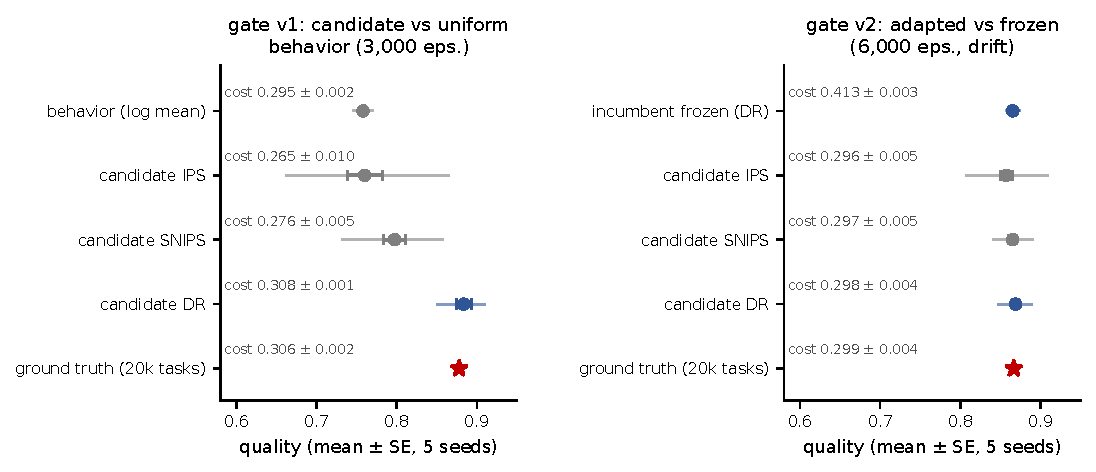
\includegraphics[width=0.9\textwidth]{figures/fig_sim_gate.pdf}
\caption{Simulator gates. Left: the constrained-GRPO candidate scored against 3{,}000 uniform-behaviour episodes on $v_1$; right: the adapted policy scored against 6{,}000 $v_2$ episodes served by the frozen policy. Points are estimates with 90\% bootstrap CIs; the star is Monte Carlo ground truth. The gate decides on DR (blue). Values from the repository README (the run's JSON outputs are not committed).}
\label{fig:sim}
\end{figure}

\begin{table}[htbp]
\centering\small
\caption{Simulator drift table (ground truth, $\lambda=0.343$). priced-BWT $=J(\text{ii})-J(\text{i})=-0.045$; recovery $=J(\text{iii})-J(\text{ii})=+0.033$.}
\label{tab:simdrift}
\begin{tabular}{lcccc}
\toprule
condition & quality & cost & within budget & $J$ \\
\midrule
(i) frozen on $v_1$ & 0.880 & 0.303 & yes & 0.776 \\
(ii) frozen on $v_2$ & 0.870 & 0.406 & no & 0.731 \\
(iii) adapted on $v_2$ (after gate) & 0.871 & 0.312 & yes & 0.764 \\
\bottomrule
\end{tabular}
\end{table}

\paragraph{Limitations.} The simulator's difficulty structure, success tables and drift event are hand-written; the run demonstrates the mechanics, not effect sizes. Single seed. The sim gate fits its direct model in-sample (buckets hold hundreds of transitions).

\subsection{CRMArena-Pro counterfactual collection}
\label{sec:crm}

\paragraph{Setup.} 50 b2b tasks (2--3 per category, all 22 categories), each run on all three tiers with a fixed continuation (\code{CONTINUE} on that tier until the agent answers, \code{ANSWER} forced at the cap), so each task's first-step tier is a contextual bandit with a fully observed reward table and the held-out value of any tier policy is an exact lookup. The log holds 150 episodes from 832 priced calls, \$17.98 under a \$21 cap; episodes average 5.0 turns and 16 of 150 hit the 12-turn cap. The behaviour is uniform over tiers (propensity $1/3$ at step 0, $1$ after). The learned decision is the first-step tier from the 43-dimensional step-0 features. Policies are trained under 5-fold category-stratified CV over task ids (train on 40, evaluate on the held-out 10, seed 0), at fixed $\lambda\in\{2,5,10\}$ per dollar with AWR+IPS, and under a budget $B=\$0.10$ with constrained GRPO on the lookup table (learned $\lambda$).

\begin{figure}[htbp]
\centering
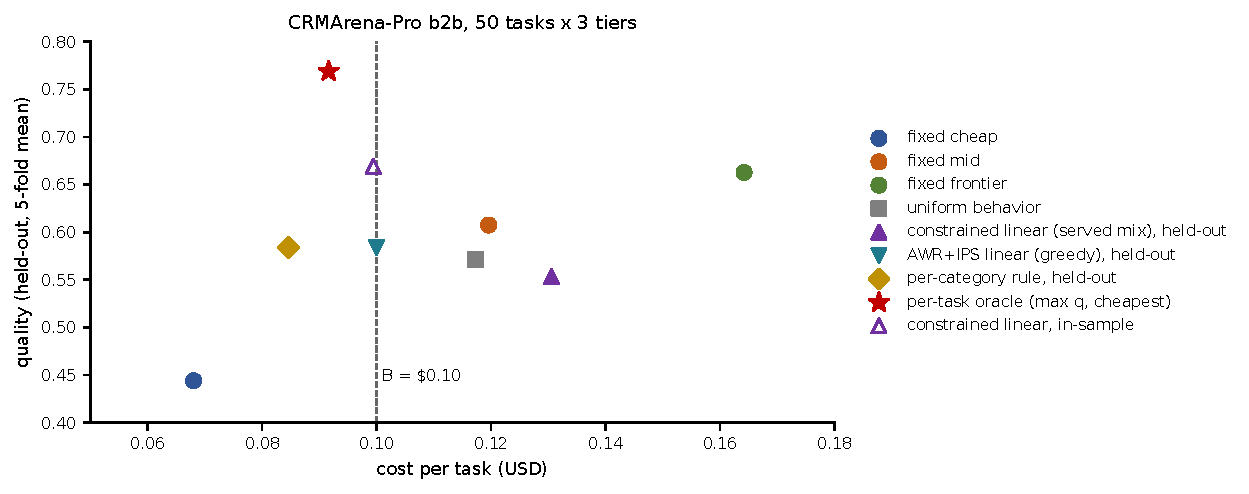
\includegraphics[width=0.78\textwidth]{figures/fig_crm_tiers.pdf}
\caption{CRMArena-Pro b2b: held-out quality against cost per task (5-fold means, exact lookups). The per-task oracle beats every fixed arm on both axes; no learned policy does. The open triangle is the constrained policy in-sample (0.669 at \$0.099), the filled one held-out (0.553 at \$0.131).}
\label{fig:crm}
\end{figure}

\begin{table}[htbp]
\centering\small
\caption{Held-out first-step tier policies on CRMArena-Pro b2b (5-fold means; cost in USD per task; across-fold SD of $J$ in brackets, 0.05--0.3 throughout, as large as the gaps between rows).}
\label{tab:crmcv}
\resizebox{\textwidth}{!}{%
\begin{tabular}{lcccc}
\toprule
policy (held-out) & $\lambda=2$: $J$ & $\lambda=5$: $J$ & $\lambda=10$: $J$ & $B=\$0.10$: quality / cost \\
\midrule
AWR+IPS linear, served (stochastic) & 0.350 [0.047] & 0.045 [0.126] & $-0.414$ [0.246] & -- \\
AWR+IPS linear, greedy & 0.384 [0.076] & 0.186 [0.126] & $-0.273$ [0.272] & -- \\
per-category plug-in rule & 0.415 [0.066] & 0.161 [0.104] & $-0.214$ [0.154] & -- \\
constrained cgrpo-lookup (iterate mix) & -- & -- & -- & 0.553 / 0.131 (over) \\
uniform behaviour & 0.337 [0.066] & $-0.015$ [0.164] & $-0.601$ [0.340] & 0.571 / 0.117 \\
fixed cheap & 0.308 [0.179] & 0.104 [0.227] & $-0.236$ [0.308] & 0.444 / 0.068 \\
fixed mid & 0.368 [0.092] & 0.010 [0.124] & $-0.588$ [0.298] & 0.608 / 0.120 \\
fixed frontier & 0.334 [0.133] & $-0.159$ [0.317] & $-0.980$ [0.633] & 0.663 / 0.164 \\
per-task oracle & 0.639 [0.056] & 0.452 [0.080] & 0.148 [0.168] & 0.769 / 0.092 \\
\bottomrule
\end{tabular}}
\end{table}

\paragraph{Results.} Table~\ref{tab:crmcv} and Figure~\ref{fig:crm}. No learned linear rule clearly beats the best fixed arm held-out: the served AWR policy has lower $J$ than the best fixed arm at every $\lambda$ ($0.350$ vs mid $0.368$; $0.045$ vs cheap $0.104$; $-0.414$ vs cheap $-0.236$), and its greedy version and the per-category rule beat the best arm by at most $0.08$, inside the fold SDs. The features memorise: AWR's $J$ at $\lambda=2$ is $0.475$ in-sample against $0.350$ held-out; the constrained policy meets the budget in-sample ($0.669$ at \$0.099) and overspends held-out ($0.553$ at \$0.131), where it is dominated by the uniform behaviour ($0.571$ at \$0.117). Even the context-free arm mixture tuned to $B$ on 40 tasks costs \$0.115 on the held-out 10. The per-task oracle reaches $0.769$ at \$0.092, beating every arm on both quality and cost: the headroom is per task, not per category, and the missing piece is an observable that predicts which tier a task needs. Repricing events (frontier $\times1.5$, cheap $\times3$), with costs recomputed from logged tokens, push the frozen all-50 policy ($\bar\lambda=1.36$/USD) over budget by $+\$0.029$ and $+\$0.035$: priced-BWT $-0.040$ and $-0.048$, in-sample recovery $+0.069$ and $+0.091$; but held-out the retrained policies still overspend (about \$0.125) and the gate on the repriced realised log \REVERT{}s all three retrains, which the held-out table says is the right call (recovery $-0.012$ for frontier $\times1.5$).

\paragraph{Limitations.} Fifty tasks, one org, one seed; one task moves a fold's quality by $0.1$. Only the first-step tier is learned, because the continuation was fixed at collection. The log holds one harness version, so version drift cannot be measured on it. Prompt caching was not used, so the roughly 5k-token system prompt is paid on every turn.

\subsection{The gate's sample-size result}
\label{sec:gatepower}

\paragraph{Setup.} The candidate is the constrained policy trained on all 50 tasks (exact value: quality $0.665$, cost \$0.0987, within $B+\mathrm{tol}=\$0.105$). The realised behaviour log is one uniformly drawn arm per task (50 episodes). The gate (cross-fitted DR, $\epsilon_q=0.03$) is run once, then over 200 independent redraws of the realised log with a 200-resample bootstrap in each.

\paragraph{Results.} On the single realised log DR estimates $0.740$ $[0.627,0.855]$ and cost \$0.0960 $[0.0750,0.1200]$; the quality criterion passes and the cost criterion fails ($0.1200>0.105$): \REVERT. On the full counterfactual log all three estimators reduce to the exact value (the weights over a task's three arms sum to 3) and the CI is pure task-sampling uncertainty from 50 tasks; the cost upper bound is still \$0.1122 and the decision is still \REVERT. Over the 200 redraws (Table~\ref{tab:redraw}, Figure~\ref{fig:gatepower}) DR halves IPS's quality RMSE ($0.048$ vs $0.094$) with 99\% coverage of its 90\% CI, but its cost CI is \$0.046 wide on average, so the candidate, whose exact cost is \$0.0013 under $B+\mathrm{tol}$, is \PROMOTE{}d in only $12/200=6\%$ of redraws. The gate errs on the safe side; buying power means more tasks or a wider tolerance. As a back-of-envelope figure (not a measurement), with CI width scaling as $1/\sqrt n$, certifying a \$0.005 margin needs a CI near \$0.01, i.e.\ roughly $20\times$ the tasks, about 1{,}000.

\begin{table}[htbp]
\centering\small
\caption{Estimators over 200 redraws of the realised CRMArena-Pro log ($n=50$, one arm per task). Cross-fitted direct model. \PROMOTE{} in 12/200 redraws (6\%).}
\label{tab:redraw}
\begin{tabular}{llcccc}
\toprule
metric & estimator & bias & RMSE & mean 90\% CI width & CI covers exact \\
\midrule
quality & IPS & $+0.011$ & 0.094 & 0.338 & 94\% \\
quality & SNIPS & $+0.001$ & 0.048 & 0.238 & 100\% \\
quality & DR & $+0.004$ & 0.048 & 0.256 & 99\% \\
cost & IPS & $+0.0001$ & 0.0114 & 0.0414 & 92\% \\
cost & SNIPS & $-0.0009$ & 0.0102 & 0.0381 & 92\% \\
cost & DR & $-0.0018$ & 0.0114 & 0.0461 & 92\% \\
\bottomrule
\end{tabular}
\end{table}

\begin{figure}[htbp]
\centering
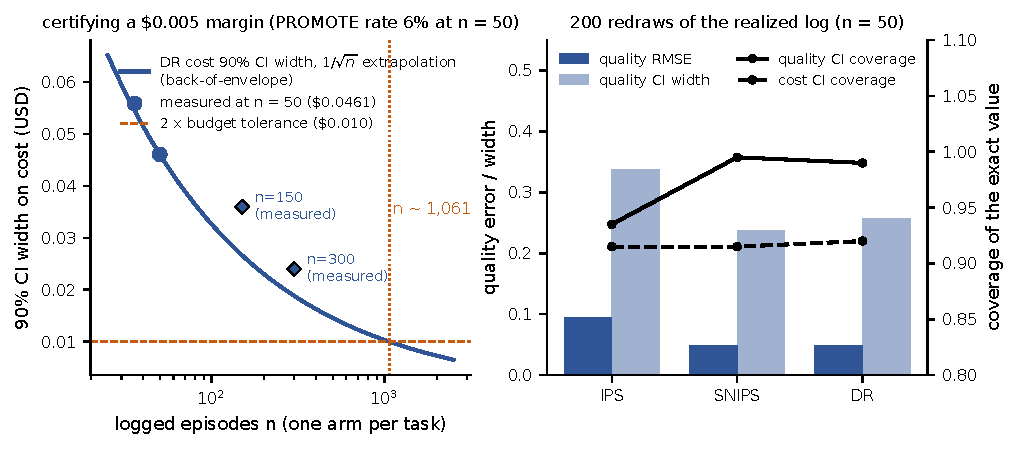
\includegraphics[width=0.9\textwidth]{figures/fig_gate_power.pdf}
\caption{Gate power. Left: the measured DR cost CI width at $n=50$ and its $1/\sqrt n$ extrapolation (a back-of-envelope, not a measurement) against twice the budget tolerance. Right: estimator RMSE, CI width and coverage over the 200 redraws.}
\label{fig:gatepower}
\end{figure}

\paragraph{Limitations.} The in-sample direct model covers $96\%/94\%$ with a $-0.006$ quality bias, a difference inside the noise at $n=50$; the redraw study reports bias and coverage empirically rather than assuming them.

\subsection{LLM controller: GRPO with LoRA on a 1.7B model}
\label{sec:llm}

\paragraph{Setup.} The controller is Qwen3-1.7B \citep{qwen3} with a LoRA adapter \citep{hu2022lora} ($r=16$ on the attention and MLP projections, bf16), trained with GRPO. The agent models stay frozen; the tiers are the arms. The prompt shows the difficulty proxy, the state, per-tier prices, the budget and the legal actions, and the completion must be exactly one tag \code{<action>TIER OP</action>}; anything else is invalid (reward $-1$, cost booked as the cheapest safe action). After the first action a fixed continuation answers on the same tier; the reward is $q-\lambda C$ with $\lambda$ learned by the same damped dual ascent, once per step from the batch mean cost. Each step generates 64 completions (8 prompts $\times$ 8 generations in phases 1 and 1b; 4 $\times$ 16 in 1c), length 16, lr $10^{-5}$, over 2{,}000 seeded sim tasks with the legal-action order shuffled per task (with a fixed order the base model only ever sampled one or two arms). Three runs on the simulator, each run once on one A100-40GB: \code{phase1} ($\lambda$ lr 0.1, $k_p$ 2.0, $\beta_{\mathrm{KL}}$ 0.02, 300 steps, 1{,}422 s, about \$0.83); \code{phase1b} (slower dual step: lr 0.02, $k_p$ 0.5, EMA 0.95; $\beta_{\mathrm{KL}}$ 0.05; entropy 0.01); \code{phase1c} (150 SFT steps on per-difficulty oracle labels at a price shown in the prompt and drawn from $\{0.0,0.1,\dots,2.0\}$, adapter merged so the KL reference is the SFT policy, then 200 GRPO steps with 16 generations, temperature 1.2, $\lambda_0=0.5$; 1{,}134 s of training plus 278 s of eval, about \$0.82). A fourth run (\code{crm\_phase2}) applies the same recipe to CRMArena-Pro fold 0 in lookup mode (574 s, about \$0.35).

\begin{figure}[htbp]
\centering
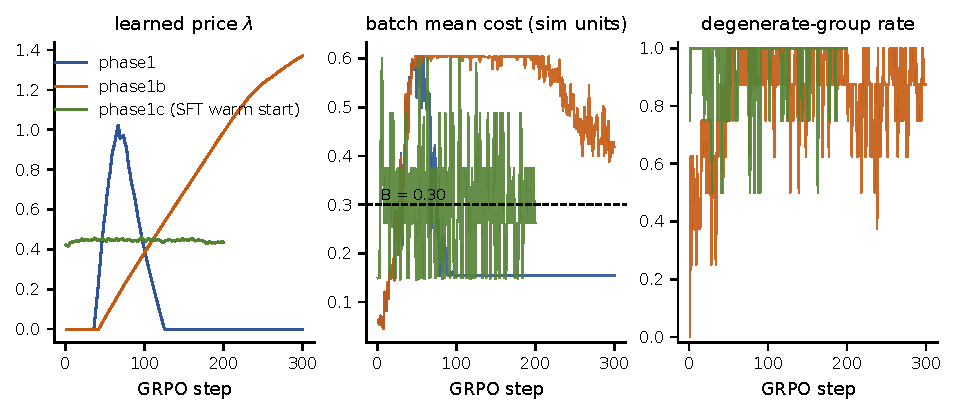
\includegraphics[width=0.9\textwidth]{figures/fig_llm_training.pdf}
\caption{GRPO training logs. \code{phase1}'s price orbits once and decays to 0 as the policy collapses onto \code{mid RETRIEVE}; \code{phase1b}'s price is still rising at step 300 while cost stays above budget; \code{phase1c}'s price settles at $\lambda\approx0.44$ with the batch cost alternating between two deterministic rules. Degenerate groups (all completions identical, hence zero advantage) dominate every run.}
\label{fig:llm}
\end{figure}

\begin{table}[htbp]
\centering\small
\caption{LLM controller on sim $v_1$ (2{,}000 fresh tasks, seed 777; budget $B=0.30$; the policy's first action then \code{ANSWER} on the same tier). ``Within'' means cost $\le B+0.02$.}
\label{tab:llm}
\resizebox{\textwidth}{!}{%
\begin{tabular}{lcccc}
\toprule
policy & quality & cost & within & invalid \\
\midrule
Qwen3-1.7B zero-shot (greedy, no adapter) & 0.586 & 0.048 & yes & 18.9\% \\
\code{phase1}, steps 100 / 200 / 300 & 0.748--0.749 & 0.155 & yes & 0\% \\
\code{phase1b}, step 100 & 0.885 & 0.603 & no & 0\% \\
\code{phase1b}, step 300 & 0.832 & 0.434 & no & 0.1\% \\
\code{phase1c}: SFT only, and GRPO steps 100 and 200 (all identical) & 0.848 & 0.330 & no & 0\% \\
linear controller (\code{policy\_v1\_sim.json}), first action only & 0.573 & 0.035 & yes & 0\% \\
fixed \code{ANSWER} on cheap / mid / frontier & 0.522 / 0.688 / 0.820 & 0.020 / 0.100 / 0.400 & yes / yes / no & 0\% \\
best deterministic per-proxy rule (easy: mid \textsc{escalate}; hard: frontier \textsc{answer}) & 0.814 & 0.250 & yes & -- \\
best randomised policy at cost exactly $B$ (LP) & 0.835 & 0.300 & yes & -- \\
\emph{derived:} \code{phase1c} served with the price drawn as in training's last 100 steps & 0.837 & 0.305 & yes & -- \\
\bottomrule
\end{tabular}}
\end{table}

\paragraph{Results.} Table~\ref{tab:llm} and Figure~\ref{fig:llm}. GRPO alone never found the budgeted optimum. \emph{Group degeneracy}: within a prompt group the completions are almost always identical, 83.5\% of groups on average in \code{phase1b}, which gives zero GRPO advantage, so the only learning signal is $\lambda$ moving the mean reward between steps and the policy jumps between near-deterministic arms instead of learning the per-proxy split. \emph{Primal--dual orbit}: in \code{phase1} the policy swings to \code{frontier RETRIEVE} (cost 0.60), $\lambda$ climbs to 1.02 by step 67, the policy collapses onto \code{mid RETRIEVE} (0.155) and $\lambda$ decays to 0 with nothing to pull it back; in \code{phase1b} $\lambda$ is still rising at step 300 (1.37) and the policy has not reached the budget. Mixing is not the bottleneck: a deterministic per-proxy rule reaches $0.814$ at $0.250$ and randomisation adds only $0.021$; what the runs failed to do is condition on the proxy. In \code{phase1c} the SFT stage reached 100\% held-out agreement with the oracle labels (1{,}000 prompts, 0\% invalid) and splits by difficulty where the oracle does; GRPO then left the policy unchanged on all 2{,}000 eval tasks (the degenerate-group rate averaged 93\% over steps 1--100 and 97\% over 101--200 even after the rollout temperature was raised from 1.2 to 1.5 at step 20). GRPO's contribution is the price: $\lambda$ settles at $0.44$ (mean $0.443$ over the last 100 steps), which is the slope at which the hard-proxy action flips. At that price the SFT policy ($J=0.702$) ties the oracle rule ($0.703$) and the LP ($0.702$). No single greedy policy meets $B=0.30$: at any one shown price the policy is a deterministic rule costing $0.33$ or $0.15$; training met the budget by alternating the shown price over time (batch cost $0.301$ and $0.296$ over the two halves), and serving can reach it by drawing the shown price (the price-conditioned analogue of iterate averaging): $0.837$ at $0.305$, derived from the two greedy rules rather than decoded end to end. On CRMArena-Pro fold 0, the SFT policy ignores the shown price (the same per-category rule at every $\lambda$, about \$0.075, under budget), so $\lambda$ fell to 0 by step 17; GRPO moved training-set quality from $0.705$ to $0.730$ and left the 10 held-out tasks unchanged at $0.700$ / \$0.073, against fixed frontier $0.700$ / \$0.142 and the fold-0 linear policy $0.590$ / \$0.143. That is one 10-task fold where one task is $0.1$ of quality and the 5-fold mean of the same category rule is $0.584$ / \$0.085 (Table~\ref{tab:crmcv}): a single draw, not evidence of generalisation or of the LLM beating the linear controller.

\paragraph{Limitations.} Each GPU run ran once; no seed variance. The phase-1 table truncates the linear policy's continuation (its first action is \code{cheap RETRIEVE} because it was trained to keep going; with its own continuation it scored $0.876$ at $0.301$ in the run that produced that file), so its row is not its real performance. Showing $\lambda$ rounded to 0.1 puts $\bar\lambda=0.443$ on the over-budget side of the flip point.

\subsection{Process-verified multi-agent orchestration}
\label{sec:mas}

\paragraph{Setup.} A planner (cheap tier) decomposes a CRM request into 1--3 sub-queries; a data worker (mid) runs one sub-query at a time through the harness's own step path; a verifier (cheap) checks a sub-result against its goal (a structural pre-check fails at \$0 on query errors); the answer is the harness's forced \code{ANSWER@mid}. After every worker step an orchestration policy chooses $\{\textsc{verify},\textsc{skip\_verify},\textsc{replan},\textsc{answer}\}\times$ tier; a fail retries the sub-query once; at most 8 role calls per episode. Fixed modes \code{always\_verify} and \code{never\_verify}, plus a uniform exploration mode with logged propensities, were run on the same 50 b2b tasks as the counterfactual log: 130 episodes (50 + 50 + 30, stopped by the ledger cap), \$10.97, \$0.084 per episode. An orchestration reward model (ORM: logistic regression and a 16-unit MLP over process features) is evaluated out of fold over tasks.

\begin{table}[htbp]
\centering\small
\caption{Decomposition against the single ReAct agent on the same 50 CRMArena-Pro b2b tasks (single-agent rows are exact lookups of the counterfactual log). The six confidentiality tasks score 0 for every system, so the ceiling is 0.88.}
\label{tab:mas}
\resizebox{\textwidth}{!}{%
\begin{tabular}{lcccc}
\toprule
system & accuracy / quality & cost / task & $J(\lambda=2)$ & $J(\lambda=5)$ \\
\midrule
single agent, fixed cheap & 0.444 & \$0.0680 & 0.308 & 0.104 \\
single agent, fixed mid & 0.608 & \$0.1196 & 0.368 & 0.010 \\
single agent, fixed frontier & 0.663 & \$0.1642 & 0.334 & $-0.159$ \\
single agent, per-task oracle (max quality, cheapest) & 0.769 & \$0.0916 & 0.586 & 0.311 \\
MAS \code{always\_verify} & 0.480 & \$0.0906 & 0.299 & 0.027 \\
MAS \code{never\_verify} & 0.461 & \$0.0821 & 0.297 & 0.051 \\
MAS \code{controller:uniform} (30 tasks, exploration) & 0.535 & \$0.0758 & 0.384 & 0.156 \\
\midrule
\multicolumn{5}{l}{\emph{Paired, same 50 tasks:} \code{always\_verify} vs \code{never\_verify}: 6 wrong$\to$right, 5 right$\to$wrong, net $+1$ ($\Delta q=+0.019\pm0.067$ SE, $+\$0.0086$).}\\
\multicolumn{5}{l}{\code{always\_verify} vs single mid: both right 19, MAS right / mid wrong 5, MAS wrong / mid right 11, both wrong 15 (net $-6$).}\\
\bottomrule
\end{tabular}}
\end{table}

\begin{table}[htbp]
\centering\small
\caption{Orchestration reward model, out of fold over tasks (130 episodes, base rate $P(\text{correct})=0.485$, base-rate Brier 0.250).}
\label{tab:orm}
\begin{tabular}{llccc}
\toprule
model & features & AUROC & Brier & ECE (5 bins) \\
\midrule
logreg & process features (default) & 0.469 & 0.281 & 0.114 \\
logreg & process $-$ verifier features & 0.451 & 0.280 & 0.140 \\
logreg & process $+$ category one-hot & 0.831 & 0.165 & 0.040 \\
mlp & process features (default) & 0.456 & 0.263 & 0.053 \\
mlp & process $+$ category one-hot & 0.831 & 0.164 & 0.035 \\
-- & category alone, no process feature & 0.821 & 0.166 & -- \\
\bottomrule
\end{tabular}
\end{table}

\paragraph{Results.} The headline is negative (Table~\ref{tab:mas}): the decomposition scores below the single mid-tier agent ($0.480$ vs $0.608$) at lower cost and is dominated on the priced frontier at both prices (by mid at $\lambda=2$, by cheap at $\lambda=5$); paired on the 50 tasks the single mid agent wins 11 and loses 5. This is the compute-matched single-agent comparison MAS-Orchestra \citep{masorchestra2026} reports as the bar, and it is not cleared. Three mechanisms are visible in the log: the plan is fixed up front by a cheap model with no data in hand while the single agent picks each query after seeing the last result; \code{never\_verify} gives the strong model about 2.7 worker turns and a forced answer against the single agent's about 5; and under \code{always\_verify} 47 of 50 episodes hit the 8-call cap because 65\% of verifier calls fail and each fail spends a retry. Verification bought $+1$ task for $+10\%$ cost, and the paired table says that is noise (6 flips each way, all through a fail and a retry). The verifier is an alarm, not a judge: it flags 24 of 26 wrong episodes ($P(\text{flag}\mid\text{wrong})=0.92$, silent failures $2/50$) and 23 of 24 correct ones ($P(\text{flag}\mid\text{correct})=0.96$), so $P(\text{wrong}\mid\text{flagged})=0.51$ against a base rate of $0.52$. The ORM (Table~\ref{tab:orm}) finds that process features carry no out-of-fold signal (AUROC $0.469$, Brier above the base rate) and the task category carries most of it (0.821 alone; 0.831 with process features), with CV over tasks so that this is category-level difficulty transferring to unseen tasks, resting on 2--3 training tasks per category. The priced-controller hook was exercised, not evaluated: AWR on the 30-episode ORM-relabelled exploration log changes nothing detectable per decision (per-decision SNIPS $0.563$ $[0.373,0.701]$ against the behaviour's $0.567$, ESS 55 of 64), and the episode-level estimate has ESS 7 of 30.

\paragraph{Limitations.} The verifier is a cheap model of the same family checking a mid model; no human process label. The 8-call cap interacts with a high-fail verifier, so a higher cap or a better verifier is a different system. Sequential sub-queries in one growing context.

\subsection{Priced Socratic self-refinement}
\label{sec:ssr}

\paragraph{Setup.} One Socratic self-refinement round \citep{ssr2025} on a CRMArena-Pro answer: a cheap probe decomposes the answer into 1--3 claims with self-reported confidences (about \$0.003, so a gate can look before it pays); each claim is re-solved by $k=2$ worker mini-episodes on the chosen tier ($\le3$ turns, the SOQL runs on the real org); a rewrite on that tier produces the refined answer; the benchmark's evaluator scores it. The initial answers are the cheap-tier episodes of the counterfactual log (already scored and paid). The run logged a tree, a refinement on every tier for every task, so every policy over $\{\textsc{stop},\textsc{refine}@\text{cheap},\textsc{refine}@\text{mid}\}$ is an exact lookup: \code{never}, \code{always\_1:t}, \code{uncertainty\_gated:$\tau$:t} ($\tau$ swept 0.3--0.9 on the minimum claim confidence), and a softmax-linear priced controller over 36 features trained by exact policy gradient on the tree (budget $B=\$0.10$ with learned $\lambda$, or fixed $\lambda\in\{2,5\}$; 5-fold CV over tasks). The run stopped at a \$14 cap: 42 tasks probed, 41 complete on both tiers, \$13.97, \$0.333 per tree against a \$0.36 estimate. One task is $0.024$ of quality.

\begin{figure}[htbp]
\centering
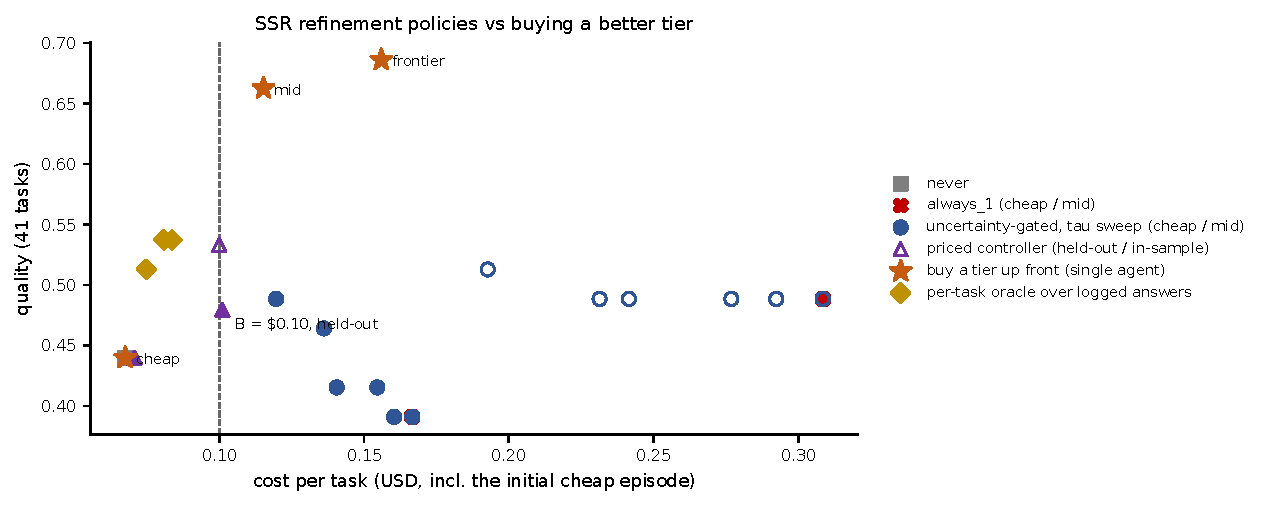
\includegraphics[width=0.82\textwidth]{figures/fig_ssr_frontier.pdf}
\caption{SSR policies on the logged tree (41 tasks, cost includes the initial cheap episode), from \code{frontier.csv}. Open circles are mid-tier gates, filled are cheap-tier. The single-agent mid arm at \$0.115 dominates every refinement policy.}
\label{fig:ssr}
\end{figure}

\begin{table}[htbp]
\centering\small
\caption{Refinement harm after one round (41 tasks). ``fix'' is wrong$\to$right out of initially wrong, ``harm'' right$\to$wrong out of initially correct.}
\label{tab:ssrharm}
\begin{tabular}{lcccccc}
\toprule
tier & changed & fix & harm & mean $\Delta q$ & round cost & worker turns \\
\midrule
cheap & 85\% (35/41) & 13\% (3/23) & 28\% (5/18) & $-0.049$ & \$0.0962 & 14.7 \\
mid & 44\% (18/41) & 13\% (3/23) & 6\% (1/18) & $+0.049$ & \$0.2380 & 13.9 \\
\bottomrule
\end{tabular}
\end{table}

\paragraph{Results.} The probe's confidence is weakly informative: AUROC $0.65$ (90\% CI $0.51$--$0.79$, $n=41$) of $1-\min$ claim confidence for predicting a wrong initial answer; the decomposer is pessimistic about everything (minimum claim confidence never above 0.75, below 0.4 on 26 of 41 tasks whether right or wrong), and the re-solve signal (AUROC 0.67 cheap, 0.55 mid) is no better than the free one; 22\% of mid worker samples are ``None''. Refinement harms as often as it helps (Table~\ref{tab:ssrharm}): a cheap round fixes 3 of 23 and breaks 5 of 18 ($\Delta q=-0.049\pm0.069$), a mid round fixes 3 and breaks 1 ($+0.049\pm0.049$), both within one SE of zero. Policies (Figure~\ref{fig:ssr}): \code{never} $0.440\pm0.078$ at \$0.068; \code{always\_1:cheap} $0.391$ at \$0.167; \code{always\_1:mid} $0.489$ at \$0.309; the best fixed cheap gate ($\tau=0.3$) $0.489$ at \$0.120; the budgeted controller $0.480\pm0.077$ at \$0.101 held-out (paired $+0.040\pm0.033$ over \code{never}, refining 20\% of tasks, $\bar\lambda=0.09$/USD because it sits under budget; $0.533$ at \$0.100 in-sample), and the fixed-$\lambda$ controllers learn \code{never}. Even the clairvoyant choice among the three logged answers per task reaches only $0.537$ at \$0.084. H1 (refine where confidence is low) is not established; H2 (always-refine is dominated under a budget) is supported, on the cheap tier by \code{never} itself; H3 (a priced gate reaches the frontier) only in the weak sense that the held-out controller sits on the frontier by learning to refine rarely. The comparison that matters is refine-the-cheap-answer against buy-mid-up-front, and buying the tier wins by a wide margin: the single-agent mid arm on the same 41 tasks scores $0.663\pm0.074$ at \$0.115; the best cheap-refinement policy at that price is $-0.174\pm0.085$ paired for $+\$0.004$; \code{always\_1:cheap} is $-0.272\pm0.099$; even refining on mid at $2.7\times$ the cost is $-0.174\pm0.092$; frontier up front ($0.686$ at \$0.156) beats every refinement policy by $0.17$--$0.30$. The sub-questions need the same schema reasoning that made the cheap agent fail, and the workers inherit it.

\paragraph{Limitations.} One round, 41 tasks, one initial arm; the $\tau$ sweep is tuned on the tasks it is evaluated on. The in-sample controller row shows what 22 category one-hots memorise on 41 tasks. Agreement with $k=2$ is weak, and no sampling parameters are sent.

\subsection{The continual orchestrator}
\label{sec:continual}

\paragraph{Harness definition.} The multi-agent structure of Section~\ref{sec:mas} is expressed as a typed harness in the terms of SkillOrchestra and EvoHarnessBench: an agent pool of typed specialists (agent id, tier, mode, stage) with modes planner, data-worker, verifier and answer; tools the orchestrator can \code{call@}; skills it can \code{engage@}; and a competence handbook over the 22 task categories (the axis the real run found carries the signal). The harness $H_t=\{\text{tools},\text{skills},\text{agents}\}$ grows monotonically by stages, $H_1\subseteq H_2\subseteq\cdots$, plus a price axis; the structure at each stage is frozen and the \emph{policy} at the decision point is what adapts, so the question is EvoHarnessBench's turned around: when $H$ expands under an orchestrator that keeps learning, what happens to the policy's backward and forward transfer, and does the gate keep it safe without making it too slow to matter? Eighteen actions: \code{delegate@data-1..4}, \code{verify@verify-1,2}, \code{replan@plan-1..3}, \code{answer@answer-1..4}, \code{call@schema\_lookup}, \code{call@aggregate\_calc}, \code{engage@soql\_aggregate}, \code{engage@date\_window}, \code{engage@decompose\_fine}; and 88 features (the real orchestrator's 66, computed by its own feature function on a view of the simulated state, plus availability flags, tools called, skills engaged, stage and a last-fail flag). Unavailable capabilities have fixed zero feature slots and zero logits, so a policy trained at stage $g$ keeps its weights when stage $g+1$ arrives.

\paragraph{Simulator and calibration.} Days of traffic under several harness changes are beyond the real-run budget, so the logged process is re-expressed as a seeded simulator whose decision points, legal-set rules and feature layout are the real orchestrator's. Every parameter is either measured from the two committed logs (130 MAS episodes, 150 single-agent episodes), with its count, or marked assumed (Appendix~\ref{app:sim}). Measured: plan-length distribution (4/22/104 of 130), worker step kinds per tier, the retry re-draw, the verifier's per-call fail rates by step kind (72 of 124 on rows, 23 of 24 on empty, 12 of 12 structural at \$0) and its episode-level $P(\text{flag}\mid\text{wrong})=0.92$ and $P(\text{flag}\mid\text{correct})=0.96$, token means per role and tier, per-category accuracy, and the configuration. Assumed: whether a rows step is the \emph{right} rows ($P(\text{good}\mid\text{rows})=0.60/0.75/0.85$ by tier), the logit slope from plan coverage to the answer (1.5, centred so \code{never\_verify} reproduces the category base rates), a task-level logit noise (sd 0.4), and everything that arrives after stage 0. On the stage-0 harness the two fixed modes reproduce the real run's process numbers (Table~\ref{tab:calib}).

\begin{table}[htbp]
\centering\small
\caption{Simulator calibration check: stage-0 harness, 1{,}000 simulated tasks per mode against the real run's 50 tasks per mode (sim / measured).}
\label{tab:calib}
\resizebox{\textwidth}{!}{%
\begin{tabular}{lccccccc}
\toprule
mode & accuracy & cost/task & role calls & verifier calls & cap hits & $P(\text{flag}\mid\text{wrong})$ & $P(\text{flag}\mid\text{correct})$ \\
\midrule
\code{always\_verify} & 0.446 / 0.480 & \$0.0894 / \$0.0906 & 7.87 / 7.88 & 2.94 / 2.94 & 95\% / 94\% & 0.95 / 0.92 & 0.93 / 0.96 \\
\code{never\_verify} & 0.459 / 0.460 & \$0.0827 / \$0.0821 & 4.75 / 4.74 & 0 / 0 & 0\% / 0\% & -- & -- \\
\bottomrule
\end{tabular}}
\end{table}

\paragraph{Pre-registered stages.} Both schedules were written down before the first full run and not changed afterwards (Table~\ref{tab:stages}). The \code{mild} schedule keeps the days and axes with smaller effects: reprice mid $\times0.8$ / frontier $\times1.2$, \code{verify-2} at $P(\text{flag}\mid\text{correct})=0.60$, \code{data-4} at rows 0.78 / good 0.75, \code{answer-4} mid-grade on 3 categories, half the tool and skill bonuses, planner v2 at 1--3 sub-queries.

\begin{table}[htbp]
\centering\small
\caption{The pre-registered default schedule: 40 days, events on days 9 / 17 / 25 / 33.}
\label{tab:stages}
\begin{tabular}{llp{1.1cm}p{9.6cm}}
\toprule
stage & day & axis & what changed \\
\midrule
g0 baseline & 1 & -- & the real run's pool: plan-1, data-1..3, verify-1, answer-1..3; list prices \\
g1 reprice & 9 & price & mid $\times0.5$, frontier $\times1.5$ \\
g2 agents & 17 & agents & $+$verify-2 (a better verifier: $P(\text{flag}\mid\text{correct})$ $0.96\to0.30$ at the same recall), $+$data-4 (database specialist, cheap), $+$answer-4 (reporting specialist, cheap) \\
g3 tools & 25 & tools & $+$schema\_lookup (the next worker step cannot error), $+$aggregate\_calc \\
g4 skills & 33 & skills & $+$soql\_aggregate, date\_window, decompose\_fine; the planner now decomposes into 1--4 sub-queries \\
\bottomrule
\end{tabular}
\end{table}

\paragraph{The day loop and comparators.} Each day is 96 seeded tasks, the same for every arm. The continual arm serves its incumbent with $\epsilon=0.1$ and logs propensities; a learner trains every day by constrained GRPO on replay from the last 5 days of logged states (60 iterations, batch 16, group 6; $\lambda$ learned against $B=\$0.090$ per task; iterate averaging), warm-started from itself; the gate (sequential DR with 200 bootstrap resamples, $\epsilon_q=0.05$, $\mathrm{tol}=\$0.005$) scores the learner against the incumbent on the log served since the last harness event (up to 5 days), with the budget net of the policy-independent prefix (planner plus first worker call, \$0.022 at list prices). An AWR+IPS variant (fixed $\lambda=2$, 200 epochs) runs the same loop. Baselines on the same traffic: \code{frozen} (the learner as of day 5, served without $\epsilon$, restricted to stage-0 actions); \code{so\_static}, a SkillOrchestra-style router whose handbook is the literal rule $\mathrm{competence}[(a,\text{category})]-\lambda_c\cdot\overline{\mathrm{cost}}[a]$ with cost tie-break, learned from the warm-up exploration traces (days 1--4) with $\lambda_c$ chosen on day 5 by episode-level SN-IPS, never updated (new capabilities scored at the handbook's prior); \code{so\_relearn}, the same router re-fitted after every stage (3 days served with $\epsilon=0.3$, then a refit and re-tune, the lag counted); \code{always\_verify}; \code{never\_verify}; and a per-stage \code{oracle} (constrained GRPO on 200 fresh exploration episodes of that stage, 300 iterations, no gate: a reference, not a proven optimum). Held-out: 150 fixed tasks per stage, simulator expected quality, never seen by the gate; $J_g=\text{quality}-\bar\lambda_g\cdot\text{cost}$ with $\bar\lambda_g$ the stage oracle's learned price (1.25 / 0.85 / 0.81 / 0.66 / 0.73 per USD for g0--g4), at which the budgeted optimum maximises the Lagrangian so $J_g$ has a ceiling and regret is well defined. Metrics follow Eq.~\eqref{eq:bwt}; in addition, hit$_j$ is the event-day policy's $J$ on stage $j$ minus on stage $j-1$, recovery$_j=R_{j,j}-R_{j-1,j}$, days-to-recover is the first day of the stage within 0.02 of the oracle, stationary $J$ the mean over the stage's last four days, and cumulative regret the sum over days 6--40 of the oracle's $J$ minus the serving policy's on the day's stage. One seed; 189 s on CPU.

\begin{figure}[htbp]
\centering
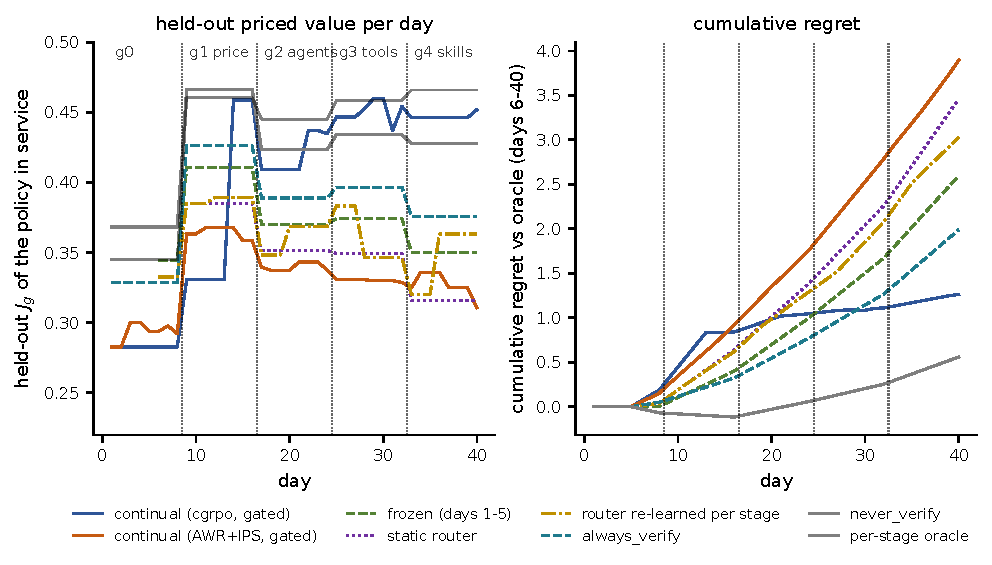
\includegraphics[width=0.95\textwidth]{figures/fig_continual_regret.pdf}
\caption{The continual orchestrator over 40 days (default schedule, from \code{days.jsonl}). Left: held-out $J_g$ of the policy in service each day; the grey upper line is the per-stage oracle. Right: cumulative regret to the oracle from day 6. The continual (cgrpo) arm is the only learned arm that recovers after every stage; \code{never\_verify} has the lowest regret of all.}
\label{fig:regret}
\end{figure}

\paragraph{Results, stated in order of importance.}

\emph{(1) The fixed mode \code{never\_verify} wins; against the learned alternatives the continual orchestrator wins on every metric.} Cumulative regret over days 6--40 (Table~\ref{tab:stream}, Figure~\ref{fig:regret}): \code{never\_verify} $0.56$, continual (cgrpo, gated) $1.26$, \code{always\_verify} $1.99$, frozen $2.60$, router re-learned per stage $3.03$, static router $3.46$, continual AWR $3.90$. \code{never\_verify}, the all-mid fixed mode, is at the oracle on g1 ($0.466$ vs $0.460$) and within $0.02$--$0.04$ on g2--g4 without learning anything: after the mid repricing, running every sub-query and the answer on the half-price mid tier is the budgeted optimum or near it in this simulator. The continual arm ends every stage within $0.001$--$0.014$ of the oracle and is the only learned arm that recovers at all (days to recover 6 / 6 / 1 / 1); the frozen controller, the static router and the re-learned router never come within $0.02$ of the oracle on any stage. The continual arm beats \code{never\_verify} only in the stationary periods of the capability-adding stages (g2 $0.429$ vs $0.423$, g3 $0.453$ vs $0.434$, g4 $0.448$ vs $0.428$) and loses that back during the recovery days. Over 5 seeds of the same configuration (Section~\ref{sec:ablation}, variant A; mean $\pm$ SE), the continual-minus-\code{never\_verify} stationary $J$ is $-0.050\pm0.011$ (g0), $-0.009\pm0.002$ (g1), $-0.014\pm0.007$ (g2), $+0.011\pm0.010$ (g3) and $+0.031\pm0.007$ (g4), and the whole-stream regret is continual $1.06\pm0.21$, \code{never\_verify} $0.74\pm0.08$, \code{always\_verify} $1.97\pm0.09$: the fixed mode's whole-stream win and the learner's margin at the last stage are both outside seed noise; the g2--g3 margins are not. The honest answer to ``does the learner beat the alternatives'' is: it beats every design-time learner, and the thing that beats it is knowing the right fixed policy in advance, which the growing pool makes less likely with every stage (the fixed mode's gap to the oracle grows from $-0.006$ at g1 to $-0.038$ at g4).

\begin{table}[htbp]
\centering\small
\caption{Per-event transfer on the default schedule (held-out $J$ of the policy in service; oracle $J$ per stage g1--g4: 0.460 / 0.445 / 0.458 / 0.466; uniform 0.351 / 0.324 / 0.317 / 0.318). Stationary $J$ per stage and BWT per stage are in Appendix~\ref{app:days} and Figure~\ref{fig:bwt}.}
\label{tab:events}
\setlength{\tabcolsep}{4pt}
\resizebox{\textwidth}{!}{%
\begin{tabular}{lcccc}
\toprule
arm & hit at event g1/g2/g3/g4 & FWT g1/g2/g3/g4 & days to recover & gap to oracle at stage end g1/g2/g3/g4 \\
\midrule
continual (cgrpo, gated) & $+.048/-.050/+.012/-.008$ & $-.020/+.085/+.130/+.128$ & 6/6/1/1 & $-.001/-.010/-.004/-.014$ \\
continual (AWR+IPS, gated) & $+.071/-.019/-.007/-.004$ & $+.012/+.016/+.014/+.006$ & --/--/--/-- & $-.102/-.107/-.130/-.155$ \\
frozen (days 1--5) & $+.067/-.041/+.004/-.024$ & $+.060/+.046/+.057/+.032$ & --/--/--/-- & $-.050/-.075/-.084/-.116$ \\
static router & $+.053/-.033/-.002/-.033$ & $+.034/+.028/+.032/-.002$ & --/--/--/-- & $-.075/-.093/-.109/-.150$ \\
router re-learned per stage & $+.053/-.041/+.015/-.026$ & $+.034/+.024/+.066/+.002$ & --/--/--/-- & $-.071/-.076/-.112/-.103$ \\
\code{always\_verify} & $+.097/-.037/+.008/-.021$ & $+.075/+.065/+.080/+.057$ & --/--/--/-- & $-.034/-.056/-.062/-.090$ \\
\code{never\_verify} & $+.098/-.043/+.011/-.006$ & $+.115/+.099/+.117/+.109$ & 1/--/--/-- & $+.006/-.022/-.024/-.038$ \\
\bottomrule
\end{tabular}}
\end{table}

\begin{table}[htbp]
\centering\small
\caption{Whole-stream summary, default schedule (mild schedule in parentheses).}
\label{tab:stream}
\begin{tabular}{lccc}
\toprule
arm & mean BWT & mean FWT & regret, days 6--40 \\
\midrule
continual (cgrpo on replay, gated, learned $\lambda$) & $+0.031$ ($+0.035$) & $+0.081$ ($+0.075$) & 1.262 (1.100) \\
continual (AWR+IPS, gated, $\lambda=2$) & $-0.006$ ($-0.005$) & $+0.012$ ($+0.002$) & 3.896 (3.668) \\
frozen (trained days 1--5) & 0 & $+0.049$ ($+0.053$) & 2.597 (1.970) \\
SkillOrchestra-style static router & 0 & $+0.023$ ($+0.025$) & 3.459 (2.902) \\
SkillOrchestra-style router, re-learned per stage & $+0.019$ ($+0.017$) & $+0.032$ ($+0.014$) & 3.029 (3.057) \\
\code{always\_verify} & 0 & $+0.069$ ($+0.062$) & 1.988 (1.731) \\
\code{never\_verify} & 0 & $+0.110$ ($+0.100$) & 0.559 (0.394) \\
\bottomrule
\end{tabular}
\end{table}

\emph{(2) The whole-stream headline is a cold-start artefact: the learner crosses \code{never\_verify} around day 22--25 and wins every stage window after that, while \code{never\_verify} falls further below the oracle at each capability stage.} Figure~\ref{fig:crossover}. Served $J$, continual minus \code{never\_verify}, by 8-day stage window: g0 $-0.073$, g1 $-0.070$, g2 $-0.021$, g3 $+0.024$, g4 $+0.035$; on the held-out sets $-0.085$, $-0.087$, $-0.004$, $+0.016$, $+0.019$. The served gap is positive from day 24 on and stays positive. Cumulative held-out regret to the oracle restricted to days 17--40 is $0.42$ (continual) against $0.68$ (\code{never\_verify}); restricted to days 25--40 it is $0.22$ against $0.50$, and every other arm is further behind (frozen $1.60$, re-learned router $1.74$, static $2.07$, AWR $2.14$ from day 25). The learner's served $J$ includes its $\epsilon=0.1$ exploration mass, a tax the fixed policy does not pay, and it still wins after the crossover. The whole deficit in the whole-stream number is the 12 days on the uniform policy before the first promotion (finding 3) plus the repricing recovery (days 9--13, where the half-price mid tier makes \code{never\_verify} the optimum before the learner has moved): \code{never\_verify} is above the reference oracle at g0 and g1 ($+0.023$, $+0.006$ on the held-out sets at stage end) and falls to $-0.022$, $-0.024$, $-0.038$ at g2--g4 as capabilities it cannot use arrive. The post-crossover margin at g4 holds over 5 seeds ($+0.031\pm0.007$, above); the stage-2+ capabilities are assumed parameters (Appendix~\ref{app:sim}), so its size is the simulator's. The same analysis is finding 2 of the repository's \code{results/mas\_continual/interpretation.md}.

\begin{figure}[htbp]
\centering
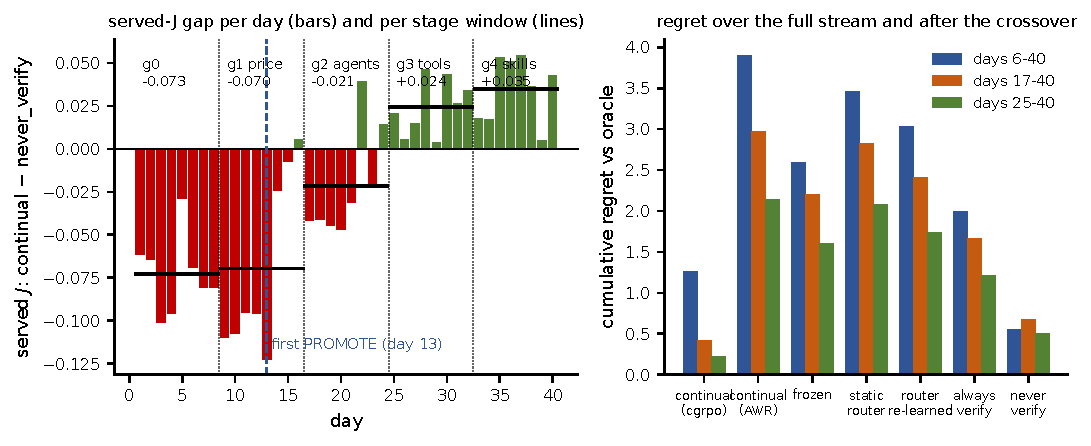
\includegraphics[width=0.95\textwidth]{figures/fig_continual_crossover.pdf}
\caption{The crossover. Left: served $J$ of the continual arm minus \code{never\_verify}, per day (bars) and averaged per stage window (black lines), with the harness events (dotted) and the first promotion (dashed, day 13). Right: cumulative held-out regret to the oracle over the full stream (days 6--40) and restricted to after the agent-pool event (17--40) and after the tools event (25--40). Both panels from \code{days.jsonl}.}
\label{fig:crossover}
\end{figure}

\emph{(3) The gate's price is larger than its benefit on this stream: 32 of 40 candidates reverted, 9 rightly and 23 as false alarms, first promotion on day 13.} Figure~\ref{fig:gatehist} and Table~\ref{tab:gatehist}. Every one of the 9 correct \REVERT{}s was a budget violation (candidate true cost \$0.095--0.101 against $B+\mathrm{tol}=\$0.095$) and no promoted candidate was bad. The DR cost estimate is the criterion that works: RMSE \$0.006 against the simulator's truth, and the set of candidates it stopped is exactly the set of over-budget candidates. The quality criterion produces the false alarms: 18 of the 32 \REVERT{}s failed on quality alone with the candidate acceptable. At $n\approx500$--$1{,}000$ logged episodes the DR quality 90\% CI is $0.20$ wide and covers the truth 63\% of the time, so a candidate whose lower bound must reach the incumbent's point estimate minus $0.05$ passes only when it is visibly better. During days 1--12 the served policy was therefore the uniform $\epsilon$-policy while the learner was already good: the frozen arm, which is the learner's day-5 snapshot, scores $0.411$ on g1 against the served incumbent's $0.247$ on day 9. This is the same sample-size finding as Section~\ref{sec:gatepower}: the cost side is certifiable at about 500 episodes a day, the quality side is not.

\begin{figure}[htbp]
\centering
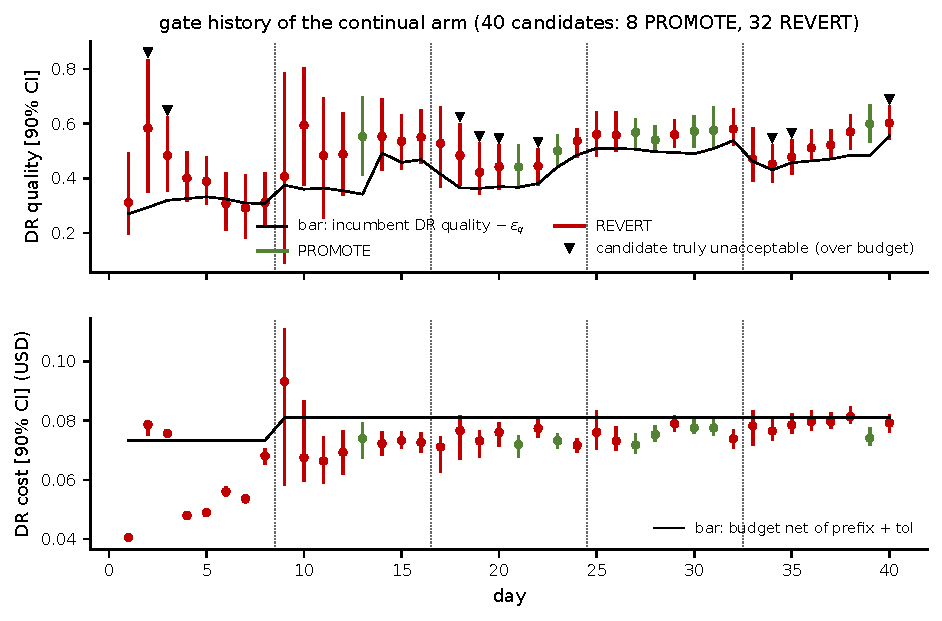
\includegraphics[width=0.88\textwidth]{figures/fig_continual_gate.pdf}
\caption{Gate history of the continual arm (from \code{gates.jsonl}). Top: DR quality with its 90\% CI against the bar (incumbent's DR quality minus $\epsilon_q$); bottom: DR cost against the budget net of the prefix plus tolerance. Green is \PROMOTE, red \REVERT; triangles mark candidates the simulator says were truly over budget. The cost criterion catches every bad candidate; the quality criterion rejects acceptable ones until they are visibly better.}
\label{fig:gatehist}
\end{figure}

\begin{table}[htbp]
\centering\small
\caption{Gate history and estimator accuracy against simulator truth (the candidate's true held-out value on the current stage), days after warm-up (35 gates, mean $n=370$ episodes per gate).}
\label{tab:gatehist}
\begin{tabular}{lcc}
\toprule
 & continual (cgrpo on replay) & continual (AWR+IPS) \\
\midrule
candidates: \PROMOTE{} / \REVERT & 8 / 32 & 14 / 26 \\
\REVERT{} right (candidate bad) / false alarm & 9 / 23 & 0 / 26 \\
\PROMOTE{} right / missed (candidate bad) & 8 / 0 & 14 / 0 \\
mean per-decision ESS / $n$ & 0.54 & 0.25 \\
mean DR quality CI width / cost CI width & 0.200 / \$0.0079 & 0.653 / \$0.0144 \\
DR quality: bias / RMSE / CI covers truth & $-0.005$ / 0.067 / 63\% & $+0.676$ / 0.809 / 6\% \\
DR cost: bias / RMSE / CI covers truth & $+0.0003$ / \$0.0061 / 54\% & $+0.0000$ / \$0.0056 / 69\% \\
per-decision SNIPS quality: bias / RMSE & $-0.020$ / 0.053 & $+0.178$ / 0.187 \\
\bottomrule
\end{tabular}
\end{table}

\emph{(4) The AWR+IPS variant is the cautionary row.} It was promoted 14 times and is the worst learned arm (stationary $J$ $0.32$--$0.36$) because the gate's sequential DR over-estimated its quality by $+0.68$ on average (coverage 6\%). AWR's exponentiated inverse-propensity weights move the policy far from the behaviour in one full-batch step; the cumulative ratios (clipped at 50) then carry the estimate with a per-decision ESS of 25\% and a bias the clip does not remove. The per-decision estimators' bias on the same candidates is $+0.18$, better but not a safe bar. The cgrpo candidates, trained on rollouts sampled from the $\epsilon$-mixed served policy, stay close to the behaviour (ESS 54\%) and the same estimator is nearly unbiased on them ($-0.005$). The gate is only as good as the overlap between candidate and behaviour, and a trainer that preserves that overlap is part of the safety story.

\begin{figure}[htbp]
\centering
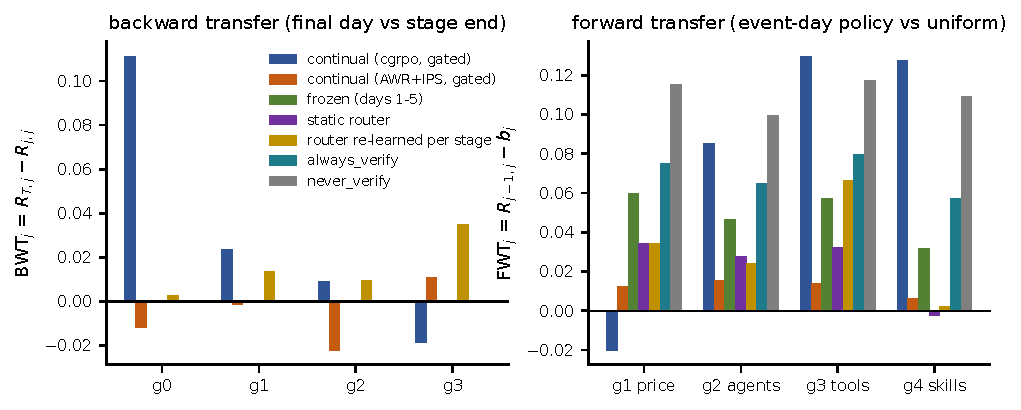
\includegraphics[width=0.9\textwidth]{figures/fig_continual_bwt.pdf}
\caption{Orchestrator-level backward and forward transfer per stage, Eq.~\eqref{eq:bwt}, computed from \code{days.jsonl}. The fixed arms have BWT 0 by construction. The continual arm's large g0 BWT is the day-8 incumbent being the uniform policy (finding 3), not transfer.}
\label{fig:bwt}
\end{figure}

\emph{(5) Orchestrator-level BWT is bounded and mostly positive.} Figure~\ref{fig:bwt}. The continual arm's BWT per stage is $+0.111$ (g0), $+0.023$ (g1), $+0.009$ (g2), $-0.019$ (g3); the mild schedule gives $+0.120$, $+0.026$, $+0.002$, $-0.009$. Later training did not undo earlier behaviour because the harness only grows: a capability that arrives at stage $g$ has a zero feature slot and a zero logit before it, and the stage-$g$ weights are still what runs where it is not legal. Contrast EvoHarnessBench's $-34.7\%$ BWT for agent-pool expansion under a fixed policy: here the pool expansion costs the fixed policies at the event (frozen hit $-0.041$, static $-0.033$ at g2) and they never recover (stationary $J$ falls from $0.411$ / $0.385$ at g1 to $0.350$ / $0.316$ at g4), while the policy that moves loses nothing on the old stages.

\emph{(6) FWT is a property of the policy in service, not of anticipation.} New capabilities arrive with zero logits, so the event-day policy is the previous stage's; the continual arm's FWT on g2--g4 ($+0.085$ / $+0.130$ / $+0.128$) exceeds the frozen arm's ($+0.046$ / $+0.057$ / $+0.032$) because it is a better policy, and the static router's FWT falls to $-0.002$ at g4 because its handbook prices unseen capabilities at a prior. Hits at the events are small for every arm except the price event, where the halved mid price lifts every mid-heavy policy by $+0.05$ to $+0.10$.

\emph{(7) The SkillOrchestra-style router is the weakest design-time baseline here, and the reason is diagnostic.} The competence of an action is the mean outcome of episodes in which it was taken, which under per-step exploration is confounded by everything else in the episode: the handbook over-selects \code{verify@verify-1} (28\% of decisions), an action the real run showed buys nothing. And $\lambda_c$ is tuned by episode-level SN-IPS of a deterministic router against $\epsilon=0.1$ traffic, whose ESS is 1--8 of 96, so the choice of $\lambda_c$ is noise and the re-learned router's $\lambda_c$ swings between 0 and 20 across stages. Re-learning per stage recovers some of the agent-pool loss ($+0.043$ at g4) at the price of three exploration days per stage, and still ends $0.07$--$0.11$ below the oracle. This is a statement about applying the competence-minus-priced-cost rule to multi-step orchestration traces with a per-step router, not about SkillOrchestra's own handbook learning from richer per-skill traces on its own benchmarks.

\paragraph{Mild-schedule sensitivity.} Figure~\ref{fig:mild} and Table~\ref{tab:stream}: the ordering is unchanged with smaller gaps (continual $1.10$, \code{never\_verify} $0.39$, frozen $1.97$, static $2.90$). In the mild run a learner exceeds the oracle at g1 (gap $+0.006$), a reminder that the oracle is a reference, not a proven optimum.

\begin{figure}[htbp]
\centering
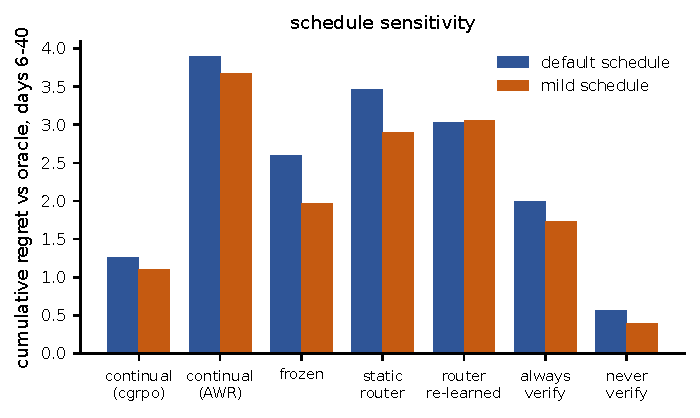
\includegraphics[width=0.55\textwidth]{figures/fig_continual_mild.pdf}
\caption{Cumulative regret under the default and the mild schedule. Same ordering, smaller gaps.}
\label{fig:mild}
\end{figure}

\subsubsection*{Verifier ablation: when does verification help?}
\label{sec:ablation}

Is ``\code{never\_verify} beats everything'' an artefact of the measured verifier (uninformative: $P(\text{flag}\mid\text{wrong})=0.92$ against $P(\text{flag}\mid\text{correct})=0.96$) and of the 8-call cap that a verify-and-retry process fills? Four controlled variants of the same 40-day stream, 5 seeds each (seeds 0--4; arms: continual cgrpo, \code{always\_verify}, \code{never\_verify}, per-stage oracle; about 220 s per run): A, the committed configuration (verify-1, cap 8), which also supplies the seed error bars above; B, the informative verify-2 for every arm from day 1 (per-call $P(\text{fail}\mid\text{good rows})$ $0.58\to0.114$, recall unchanged); C, B plus cap 12; D, C plus verifier calls exempt from the cap. Served numbers are means over all 40 days (the fixed modes do not learn); $J$ uses the stage oracle's $\bar\lambda_g$.

\begin{table}[htbp]
\centering\small
\caption{Verifier ablation: \code{always\_verify} minus \code{never\_verify}, served, mean $\pm$ SE over 5 seeds.}
\label{tab:ablation}
\resizebox{\textwidth}{!}{%
\begin{tabular}{lcccccc}
\toprule
variant & $\Delta$ expected quality & $\Delta J$ & $\Delta$ cost / task & cap hits (always) & retries / ep. (always) & verifier calls / ep. (always) \\
\midrule
A: verify-1, cap 8 (committed) & $-0.033\pm0.001$ & $-0.036\pm0.001$ & $+\$0.0036$ & 95\% & 0.89 & 2.94 \\
B: verify-2 for every arm & $-0.004\pm0.001$ & $-0.007\pm0.001$ & $+\$0.0030$ & 91\% & 0.64 & 2.90 \\
C: B + cap 12 & $+0.029\pm0.001$ & $+0.011\pm0.001$ & $+\$0.0148$ & 9\% & 0.76 & 3.65 \\
D: C + verifier exempt from cap & $+0.028\pm0.001$ & $+0.010\pm0.001$ & $+\$0.0148$ & 0\% & 0.77 & 3.64 \\
\bottomrule
\end{tabular}}
\end{table}

\begin{figure}[htbp]
\centering
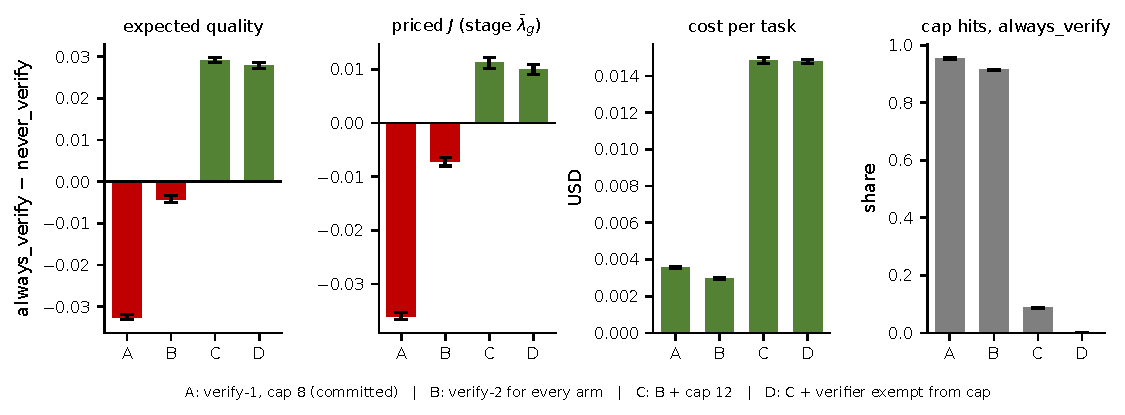
\includegraphics[width=0.95\textwidth]{figures/fig_ablation_verifier.pdf}
\caption{Verifier ablation (from the ablation summary file): \code{always\_verify} minus \code{never\_verify} in expected quality, priced $J$ and cost, and \code{always\_verify}'s cap-hit share, under the four variants; bars are means over 5 seeds with SE. The sign flips only when the verifier is informative \emph{and} the retries do not come out of the plan's call budget.}
\label{fig:ablation}
\end{figure}

Table~\ref{tab:ablation} and Figure~\ref{fig:ablation}. Under the committed configuration verification \emph{hurts}: \code{always\_verify} is below \code{never\_verify} by $0.033\pm0.001$ in expected quality and $0.036\pm0.001$ in $J$ for $+\$0.0036$ per task, consistent with the real run's $+1$ task ($+0.019\pm0.067$ SE at $n=50$). The informative verifier alone (B) closes the gap to $-0.004\pm0.001$ but does not reverse it, because 91\% of \code{always\_verify} episodes still hit the cap and the plan is truncated. Raising the cap to 12 (C) flips the sign: $+0.029\pm0.001$ quality and $+0.011\pm0.001$ $J$ for $+\$0.0148$ per task ($+18\%$), with 3.65 verifier calls and 0.76 retries per episode and 9\% cap hits (the stage-4 four-step plans). Exempting verifier calls from the cap (D) changes nothing beyond removing the last cap hits ($+0.028$ / $+0.010$): with one retry per sub-query a three-step plan already fits in 12 calls. Stated plainly: verification helps only when the verifier's fail is informative \emph{and} the retry does not come out of the plan's call budget, and then it is worth about $+0.03$ accuracy for $+18\%$ cost, a priced gain of $+0.01$ $J$ at the stage prices. Under C and D the fixed \code{always\_verify} costs \$0.098--0.105 per task, above the learner's $B+\mathrm{tol}=\$0.095$, so it can exceed the budget-constrained oracle at a stage (g1 in C: $0.443$ vs $0.434$); the learner's verify share rises from $0.03$--$0.09$ (A) to $0.10$--$0.13$ (B--D) of its decisions and no further, and within budget it still ends the last stage above \code{never\_verify} under every variant (g4: A $+0.031\pm0.007$, B $+0.017\pm0.011$, C $+0.016\pm0.007$, D $+0.013\pm0.010$). The whole-stream regret ordering under C/D is \code{always\_verify} $0.30$ $<$ \code{never\_verify} $0.60$ $<$ continual $1.05$--$1.20$: at a verifier worth using and a cap that does not truncate, the right fixed mode is \code{always\_verify}, it is over budget, and the budgeted learner is third, its cold start still the whole deficit. Two caveats. The informative verifier's episode-level $P(\text{flag}\mid\text{correct})$ in the simulator is $0.71$, not the $0.30$ its per-call parameter was derived from, because correct episodes still contain empty and wrong steps that are rightly flagged; the per-call parameter is what the ablation sets. And the effect size rests on the assumed link from a step's latent quality to the answer.

\begin{table}[htbp]
\centering\small
\caption{The real log (130 MAS episodes): what a flagged step's retry did. Observation kind before the flag (rows) against after the retry (columns).}
\label{tab:retry}
\begin{tabular}{lcccccc}
\toprule
before $\to$ after & rows & empty & error & invalid & respond & total \\
\midrule
rows & 26 & 2 & 5 & 0 & 0 & 33 \\
empty & 5 & 7 & 0 & 1 & 0 & 13 \\
error & 5 & 1 & 0 & 0 & 0 & 6 \\
invalid & 0 & 0 & 0 & 0 & 1 & 1 \\
\bottomrule
\end{tabular}
\end{table}

The real log gives the per-step number beside the per-episode one (Table~\ref{tab:retry}): 107 verifier fails, 53 followed by a retry of the same sub-query (the rest hit the cap or the one-retry limit). The retry changed the observation kind in 10 of 53 cases (19\%), always from empty/error to rows: a flagged empty, error or invalid step became rows in 10 of 20 cases, so the retry does repair malformed or empty steps; but 33 of the 53 retries were of a step that had returned rows, and 26 of those returned rows again. When the retried step was verified again it passed 11 of 47 times (23\%) against 42 of 114 (37\%) for first attempts. Paired with \code{never\_verify} on the same tasks, the 44 \code{always\_verify} episodes that retried flipped 6 wrong$\to$right and 5 right$\to$wrong, with 16 unchanged right and 17 unchanged wrong (25\% flipped, symmetric). Per step and per episode say the same thing: the measured verifier's flag is not information about correctness.

\paragraph{What this does not show.} Effect sizes are the simulator's: the stage-2+ capabilities are assumed, as is the link from a worker step's latent quality to the answer. One schedule plus a mild one; the all-arms run is one seed, with 5-seed error bars for the continual, \code{always\_verify}, \code{never\_verify} and oracle arms from the ablation of Section~\ref{sec:ablation}. The per-stage oracle is constrained GRPO on fresh exploration, not a proven optimum. Nothing here calls an API; Phase B (the real-run protocol) is a plan with a cost table (Section~\ref{sec:phaseb}).

\subsection{The same analysis at 150 tasks}
\label{sec:crm127}

After the 50-task results above, the collection was resumed on the same seeded sample to its full 150 tasks (450 episodes, every task on every tier; \$59.90 cumulative on the ledger; one interruption at 128 tasks when the API account's credit balance ran out, resumed without loss). Everything in Section~\ref{sec:crm} was re-run on that log with the same code and folds (\texttt{results/crmarena\_150/}; an intermediate run at 127 tasks is kept in \texttt{results/crmarena\_127/} and agrees in every ordering).

\begin{table}[h]\centering\small
\begin{tabular}{lrrr}\toprule
held-out, 5-fold ($\lambda=2$ per dollar) & quality & cost/task & $J$ [fold SD] \\\midrule
fixed cheap & 0.463 & \$0.060 & 0.344 [0.027] \\
fixed mid & 0.533 & \$0.120 & 0.294 [0.107] \\
fixed frontier & 0.616 & \$0.143 & 0.329 [0.115] \\
AWR+IPS linear, greedy & 0.597 & \$0.088 & 0.421 [0.081] \\
\textbf{per-category rule (train-fold argmax)} & \textbf{0.623} & \textbf{\$0.082} & \textbf{0.460 [0.094]} \\
constrained, $B=\$0.10$, greedy of the mix & 0.644 & \$0.105 & 0.559 [0.080] at fold $\bar\lambda$ \\
per-task oracle & 0.711 & \$0.057 & 0.597 [0.040] \\\bottomrule
\end{tabular}
\caption{CRMArena-Pro b2b at 150 tasks: held-out tier policies. The learned per-category policy beats every fixed arm held-out on quality and cost at once; the constrained controller exceeds frontier-tier quality at 27\% less cost, at its budget.}
\label{tab:crm150}
\end{table}

Three things changed with three times the data. (1) \emph{The learned policy wins held-out.} At 50 tasks no learned controller clearly beat the best fixed arm; at 150 the per-category rule's $J$ of 0.460 is 0.12 above the best fixed arm (cheap, 0.344), and the constrained controller's 0.644 quality at \$0.105 beats the frontier tier's 0.616 at \$0.143. The margin over the best fixed arm is a little over one fold SD, so this is a consistent ordering rather than a certified gap; the category feature stopped memorising once each category held six or seven tasks instead of two or three. (2) \emph{The gate's answer now depends on the draw, which is the point.} On the seed-0 realised one-arm log the DR estimate for the all-task constrained policy is 0.693 [0.584, 0.757] in quality and \$0.091 [0.078, 0.101] in cost, and the gate \PROMOTE{}s; on a second realised draw the cost upper bound is \$0.108 and it reverts. Over 200 redraws the promotion rate is 10\% (6\% at 50 tasks, 8\% at 127). A single promotion at this sample size is a one-in-ten event, so the redraw rate, not the seed-0 decision, is the number to report; the cost interval is still about 0.023 wide against a 0.005 margin, and the thousand-task estimate of Section~\ref{sec:gatepower} stands. (3) The tier means moved as tasks were added (frontier 0.663 $\to$ 0.616, mid 0.608 $\to$ 0.533, the oracle 0.769 $\to$ 0.711): the 50-task sample was an easy draw, which is the sample variation of Section~\ref{sec:followups} seen from the other side, and the reason the held-out comparison, not the tier table, is the result.

\paragraph{What more tasks would buy, left to the next step.} The collection stops at the 150-task seeded sample. Two extensions are costed from the measured rate of about \$0.41 per task across the three tiers and left for the next stage of the project. At \emph{200 tasks} (about \$30 more) each category holds six to nine tasks, which tightens the per-category policy's fold variance, and the gate's cost interval narrows from about 0.036 to about 0.029: the held-out ordering would not change, and the gate would still revert on cost. At \emph{300 tasks} (about \$70 more) the interval reaches about 0.023 and the promotion rate over redraws should move into the ten-to-fifteen percent range; this is also the first scale at which the category-difficulty finding of Section~\ref{sec:mas} could be checked on the single-agent log. Certifying the \$0.005 margin itself remains a thousand-task matter under the $1/\sqrt{n}$ assumption, and the full B2B split (2,140 tasks, roughly \$880) is the ceiling of what this benchmark can offer without B2C.

\subsection{Three follow-up experiments: delegation credit, meta-learned initialisation, and a skill handbook}
\label{sec:followups}

\paragraph{RAO-style delegation credit (negative).} We added the node reward of \citet{rao2026} to the continual orchestrator's trainer: for a \texttt{delegate} decision, the per-decision reward is the episode's priced outcome plus $\lambda_d$ times the mean success of the sub-call it spawned, with a leave-one-out baseline anchored on the root reward. Over five seeds on the committed simulator and schedule, delegation share rose at every stage (from 0.17/0.44/0.50/0.51/0.55 across the five stages without credit to 0.26/0.47/0.57/0.62/0.62 with $\lambda_d{=}0.5$) and served regret over days 6--40 rose from $0.94\pm0.27$ to $1.74\pm0.18$; stationary priced $J$ fell by 0.02--0.04 at every stage after the baseline. Because the credit mode also changes the baseline, we ran the same mode with $\lambda_d{=}0$: regret $0.99\pm0.24$ and unchanged shares. The credit, not the baseline, buys over-delegation. The learner without credit already delegated to new specialists from the stage they appeared; a bonus outside the baseline turns that into a habit.

\paragraph{Meta-learned controller initialisation (positive, caveated).} The learner's deficit against the fixed policy was its cold start. Following the meta-learned initialisation of \citet{tandon2025e2ettt}, we learned the controller's initial weights by a first-order meta-loop over the simulator's stage definitions $g_0$--$g_3$ (never $g_4$, never a held-out set; audited per run), then ran the continual arm from that initialisation. Over five seeds, served regret over days 6--40 fell from $1.06\pm0.21$ to $0.47\pm0.08$ (paired $-0.59\pm0.15$) and over days 17--40 from $0.76\pm0.18$ to $0.43\pm0.07$; the learner now has lower regret than \texttt{never\_verify} ($0.74\pm0.08$) on the full stream. The gain comes from what is served before and between promotions, not from earlier promotion (first-promotion day unchanged at $5.2$ in this arm set), and there is no gain on $g_4$, the one stage the meta-initialisation never saw. The caveat is structural: the initialisation was trained on the simulator's own stage definitions; on real traffic it would have to be learned from past harness generations only, and whether the gain survives that is untested.

\paragraph{Skill handbook for the cheap tier (null, with the control that showed it).} The cheap tier scores 0.444 on the 50 real tasks because it fails schema reasoning, while the mid and frontier tiers solved many of the same tasks. We distilled per-category procedural notes from those successful SOQL episodes with the mid-tier model as writer (leave-one-task-out, so no task saw notes from its own solution; 49 writer calls, \$0.27) and served the cheap tier with the notes in its prompt (\$2.39). Quality rose to 0.581 ($+0.137\pm0.070$ paired). But the 14 tasks that received no notes improved by the same amount as the 36 that did, so we re-ran the cheap tier with no notes: 0.561, a difference from the skilled arm of $+0.020\pm0.067$. The handbook did nothing measurable; the original 0.444 was a low draw. What survives is the size of that draw: the same tier on the same 50 tasks moved by $+0.117\pm0.062$ between two runs a day apart, which is as large as the gap between tiers in Section~\ref{sec:crm}, and a second, independent reason the gate of Section~\ref{sec:gatepower} refused to certify a margin at this sample size.

\section{Discussion}

\paragraph{The signal is the bottleneck.} The same pattern appears in every experiment. On CRMArena-Pro the per-task oracle is far above every arm, but the only observable the controller has at step 0 is the category, and with 2--3 tasks per category it memorises (Section~\ref{sec:crm}). The orchestration reward model finds that process features carry no out-of-fold signal while the category alone has AUROC 0.82 (Section~\ref{sec:mas}); the verifier flags nearly everything; the self-refinement probe barely sees whether the cheap answer is wrong (AUROC 0.65), so the best priced policy is ``mostly do not refine'' (Section~\ref{sec:ssr}). The LLM controller's GRPO stage had no advantage signal because its rollout groups were identical, and what it did learn was the price (Section~\ref{sec:llm}). In the continual study the gate's quality criterion has too little signal at $n\approx500$ to tell an acceptable candidate from the incumbent, while the cost criterion, whose signal is a sum of logged dollars, works (Section~\ref{sec:continual}). The learners are not the limiting factor; the observables and the sample sizes are. On this benchmark the right orchestration signal is known before the first call, and that argues for investing in observables (a verifier trained on logged (task, answer, score) triples; the mid arm's own answer as a check) before investing in policy classes.

\paragraph{When does a learned orchestrator earn its keep?} Only when a harness change moves the right fixed policy. On the stream of Section~\ref{sec:continual}, the capability-adding stages are where the continual arm's stationary $J$ exceeds the best fixed mode, and they are also where the fixed modes' gap to the oracle grows ($-0.006\to-0.038$ for \code{never\_verify}; frozen $0.411\to0.350$). A repricing moves the fixed policy's cost but not its ranking; a new specialist or tool moves the ranking, and only a policy that can see the new capability can use it. If the harness is stable and someone knows the right fixed mode, the learner's whole-stream regret (1.26) is its cold start, its recovery days and its gate delays, and the fixed mode (0.56) wins; once the pool has grown past what the fixed mode can use (from day 25: 0.22 against 0.50; g4 margin $+0.031\pm0.007$ over 5 seeds), the learner wins while paying an exploration tax the fixed mode does not. And which fixed mode is right depends on the harness: with an informative verifier and a cap the retries do not consume, it is \code{always\_verify}, over budget, and the budgeted learner is third (Section~\ref{sec:ablation}). The decision to deploy a learned orchestrator is therefore a decision about how often the harness will change in ways that re-rank the fixed policies, which is exactly what the design-time harness-evolution work predicts will be often.

\paragraph{Gate power against day size.} With binary outcomes and sequential ratios, the DR quality interval is about $\pm0.04$ or wider at $n\approx500$ ($\epsilon_q=0.05$ was needed because the core default of $0.03$ rejects the incumbent against itself at this $n$), while the cost interval is \$0.008 wide and its criterion is the binding one. Two things follow for a real deployment: certify cost and treat quality as a floor against regression, not as an improvement test; and keep the candidate close to the behaviour (the cgrpo arm's ESS of 54\% against AWR's 25\%), because the estimator's bias, not its variance, is what promoted the bad arm.

\paragraph{What Phase B would need.}
\label{sec:phaseb}
The same loop on the real orchestrator: days of 20 b2b tasks, the learner trained with AWR+IPS on the day's log (no replay exists on the real harness) and gated with the per-decision estimators, held-out evaluation by re-serving a fixed 20-task set per stage. Stages that can be induced for real: a repricing (free, costs recomputed from logged tokens); a better verifier (swap its prompt or tier; a mid verifier call is about \$0.002 against \$0.001); a new worker or answer backbone (any priced model); a worker swap by tier; a schema-lookup tool (one describe call) or a local aggregation tool (about \$0); skills as steering text (tokens only). Costs from the measured \$0.084 per episode are in Table~\ref{tab:phaseb}. A \$0.005 margin on a \$0.09 budget needs about 1{,}000 logged episodes to certify, so at 20 tasks a day the cost criterion would run on a rolling window and still be underpowered, and the quality criterion at $\epsilon_q=0.05$ needs on the order of 500 episodes. The honest Phase B at \$50 measures the mechanics (what the learner serves, what the gate does, the frozen policy's hit at each stage) rather than certifying improvements.

\begin{table}[htbp]
\centering\small
\caption{Phase B cost table (from the measured \$0.084 per episode; \$0.076 under mixed-tier exploration). Per day of 20 tasks, one policy, about \$1.70; the two fixed baselines add \$3.40.}
\label{tab:phaseb}
\begin{tabular}{lcc}
\toprule
protocol & episodes & estimate \\
\midrule
10 days $\times$ 20 tasks $\times$ 1 served policy & 200 & \$17 \\
the same with \code{always\_verify} and \code{never\_verify} on every day & 600 & \$50 \\
20 days $\times$ 20 tasks $\times$ 1 policy, two induced stages, held-out re-serves (20 tasks per stage) & 460 & \$39 \\
40 days $\times$ 20 tasks $\times$ 1 policy, four stages, held-out re-serves & 900 & \$76 \\
40 days, four stages, with the two fixed baselines & 2{,}500 & \$210 \\
\bottomrule
\end{tabular}
\end{table}

\section{Limitations and threats to validity}

\begin{itemize}
\item \textbf{Fifty tasks.} The real-harness evidence is one b2b collection of 50 tasks (2--3 per category); every held-out number is a mean over 10 tasks per fold, one task is $0.1$ of quality, and the across-fold SDs are as large as the differences between policies. The MAS run has 130 episodes on the same 50 tasks; the SSR run 41 tasks. The negative results for the linear controller, the ORM and the refinement gate are statements about this sample size and these observables, not about the approaches.
\item \textbf{Seeds.} The simulator pipeline uses one seed per stage, the CRMArena folds one split, and each GPU run ran once; the continual study's all-arms run is one seed per schedule, and only the verifier ablation (continual, the two fixed modes and the oracle; Section~\ref{sec:ablation}) reports 5-seed error bars. The router and AWR arms carry no seed variance.
\item \textbf{Simulators calibrated to the project's own logs.} The sim of Section~\ref{sec:sim} is hand-written. The continual simulator's process statistics are measured on 130 episodes, but the link from a step's latent quality to the answer and every capability that arrives after stage 0 are assumed (Appendix~\ref{app:sim}); the transfer effect sizes are the simulator's, not CRMArena's. The calibration check reproduces the fixed modes' cost and call counts but lands accuracy at $0.446/0.459$ against $0.480/0.460$, because the simulated verifier is uninformative, as the measured one is.
\item \textbf{Assumed stage parameters.} $P(\text{good}\mid\text{rows})=0.60/0.75/0.85$ by tier; coverage-to-answer logit slope 1.5; task-level logit noise sd 0.4; \code{verify-2} at $P(\text{flag}\mid\text{correct})=0.30$ with the same recall; \code{data-4} at rows 0.85 / good 0.80; \code{answer-4} mid-grade on 8 categories; \code{schema\_lookup} removes error mass from the next step; \code{aggregate\_calc} adds $+0.34$ coverage on aggregation categories; the three skills add $+0.15$ $P(\text{good}\mid\text{rows})$ on their categories or re-plan into 3--4 sub-queries; planner v2 plan length $(0.0,0.1,0.4,0.5)$. Tools and skills are priced as a verifier-sized cheap call (711/62 tokens).
\item \textbf{The SkillOrchestra baseline is the literal rule, not their system.} Competence minus $\lambda_c$ times mean logged cost, over task categories as skills, learned from per-step exploration traces of a multi-step orchestrator. Their handbook learning from richer per-skill traces on their own benchmarks is not reproduced.
\item \textbf{The oracle is a reference.} Constrained GRPO on fresh exploration with more iterations, not a proven optimum; regret can be slightly negative.
\item \textbf{Gate design.} The sim gate fits its direct model in-sample; the bandit gate cross-fits by task; the continual gate uses the sequential DR with cumulative ratios clipped at 50, whose bias on far-from-behaviour candidates is what finding (3) exposes.
\item \textbf{Data terms.} CRMArena-Pro is CC BY-NC 4.0 (research use), fetched at setup and not copied; the committed trace is a derived research artefact under the same terms (Appendix~\ref{app:license}).
\end{itemize}

\section{Related work}

\paragraph{Cost-aware routing.} FrugalGPT \citep{frugalgpt2023} cascades models by a learned score to cut cost; RouteLLM \citep{routellm2024} learns a router between a strong and a weak model from preference data; xRouter \citep{xrouter2025} trains a cost-aware orchestration system with reinforcement learning. These choose a model per query at the first turn; this report prices every decision point inside a frozen harness, learns the price as a dual variable against a budget, and gates deployment off-policy.

\paragraph{Self-evolving agent systems and the deployment seam.} A recent position paper from the AReaL group \citep{areal2} argues that enterprise self-evolving agents are blocked not by RL algorithms but by systems: a step-level episode data protocol, a data proxy that turns production workloads into governed learning material, and a unified \emph{evolution control plane} that selects, from episode statistics, drift indicators and cost, among memory updates, skill updates, harness edits, weight updates, rollback or no-op, each behind replay-first evaluation, regression tests and canary rollout. That is the architecture this report instantiates in part: the gate of Section~\ref{sec:gatepower} is a measured, interval-valued form of their replay-first check; priced backward and forward transfer are the drift indicators they call for; and the continual orchestrator of Section~\ref{sec:continual} is a per-request learner inside the harness surface they name, with the harness-edit surface left to the slow loop. Their prototype realises the weight-update path by redirecting deployed agents' inference calls through managed workers, the same seam that Agent Lightning \citep{agentlightning} uses to make training harness-agnostic through a proxy that emulates the inference APIs; placing the controller in that proxy is the deployment path we would take, since tier choice, verification and stopping are decisions at the API boundary, while replan and delegation still need a hook inside the orchestrator. Production precedent for the cadence exists: online RL after deployment has shipped with checkpoints refreshed from user interaction every few hours.

\paragraph{Recursive delegation and priced effort.} Recursive Agent Optimization \citep{rao2026} trains agents that spawn instances of themselves through a \texttt{launch\_subagent} call, with a local node reward equal to the node's own success plus $\lambda_d$ times the \emph{mean} success of its children (averaging rather than counting, which removes the incentive to spawn), a leave-one-out baseline anchored on the root reward, and depth-level inverse-frequency weighting so that deep sub-tasks do not dominate the update. Four points carry over. First, that node reward is the principled process reward for the delegate action of Section~\ref{sec:mas}, where our process rewards were definitional; we adopt its form in the continual study. Second, depth weighting is the recursive counterpart of the per-decision estimators used here. Third, delegation in RAO is unpriced: depth and step caps stand in for a budget, so adding $\lambda\cdot\mathrm{cost}$ and $\mu\cdot\mathrm{latency}$ to the node reward (their sequential case runs $18\times$ slower in wall-clock) is the one-line extension that turns the caps into a learned price, and the comparison it sets up is in-weights delegation against controller-side delegation at equal cost. Fourth, RAO's generalization from medium to hard tasks concerns the learned decomposition skill, not drift of the harness around it, which is what the transfer metrics here measure. On the shaping of the price itself, the Composer~2 report describes a nonlinear effort penalty over tokens, tool calls and turns whose slope is steeper on easy tasks than on long-horizon ones; the objective here uses a single linear $\lambda$, and a difficulty-conditioned price, $\lambda$ per task category or a concave cost curve, is a direct extension that the 50-task log is too small to fit.

\paragraph{Contextual bandits in production.} The Decision Service \citep{agarwal2016decisionservice} and Horizon \citep{gauci2018horizon} established the logging discipline (propensities with exploration), the offline evaluation \citep{li2011unbiased,bottou2013counterfactual} and the promotion workflow that the gate here follows; the estimators are those of \citet{dudik2011dr,jiang2016dr,thomas2016magic,swaminathan2015snips}, with cross-fitting after \citet{chernozhukov2018dml}.

\paragraph{Test-time compute and self-refinement.} Socratic Self-Refine \citep{ssr2025} decomposes an answer into verifiable sub-questions and rewrites where confidence is low; the uncertainty signals (verbalised confidence, sample agreement) follow \citet{verbalizedconf2025}. Section~\ref{sec:ssr} treats how much of it to buy per request as a priced decision and finds that, on a CRM benchmark, a better tier up front dominates.

\paragraph{Process verification and reward modelling for multi-agent systems.} MAS-ProVe \citep{masprove2026} studies process-level verification of multi-agent executions; reward modelling for orchestration \citep{rmorchestration2026} scores episodes to train orchestrators; MAS-Orchestra \citep{masorchestra2026} asks when a multi-agent system beats a compute-matched single agent. Section~\ref{sec:mas} measures all three on one log and finds the verifier uninformative, the process features without out-of-fold signal, and the single agent ahead.

\paragraph{Harness evolution and continual-learning metrics.} The design-time line \citep{dgm2025,gepa2025,darwinx2026,metaharness2026,envharness2026,harnessx2026} and EvoHarnessBench \citep{evoharnessbench2026} evolve or grow the harness; SkillOrchestra \citep{skillorchestra2026} learns a static competence router. The BWT/FWT definitions are those of \citet{lopezpaz2017gem}, applied here to a priced objective at the orchestrator level.

\paragraph{Offline and constrained RL.} CQL \citep{kumar2020cql} and IQL \citep{kostrikov2021iql} are the standard pessimistic offline learners; AWR \citep{peng2019awr} is the simpler weighted-regression trainer used here with inverse propensities; GRPO \citep{shao2024grpo} supplies the group-relative advantage; the learned price follows RCPO \citep{tessler2018rcpo} and the PID-Lagrangian \citep{stooke2020pid}, with iterate averaging after \citet{nedic2009saddle}.

\section*{Acknowledgements}
The authors of CRMArena-Pro released the benchmark, its prompts, evaluator and read-only sandbox that made the real-harness experiments possible.

{\small
\bibliographystyle{plainnat}
\bibliography{refs}}

\appendix

\section{Estimator derivations}
\label{app:estimators}

\paragraph{Unbiasedness of per-decision IPS.} For a logged episode drawn from $\mu$, and any step $t$, $\E_\mu[\rho_{0:t}\,r_t]=\sum_{a_{0:t}}\prod_{k\le t}\mu(a_k\mid s_k)\prod_{k\le t}\frac{\pi(a_k\mid s_k)}{\mu(a_k\mid s_k)}\,r_t=\E_\pi[r_t]$, whenever $\mu(a\mid s)>0$ wherever $\pi(a\mid s)>0$; the $\epsilon$-mixture of Eq.~\eqref{eq:policy} guarantees the support condition for every served log. Summing over $t$ gives Eq.~\eqref{eq:ips}. The clip at $\rho_{\max}$ trades this unbiasedness for variance.

\paragraph{The doubly-robust decomposition.} Write $\delta_t=r_t+\hat V(s_{t+1})-\hat Q(s_t,a_t)$, the temporal-difference residual of the direct model under the candidate. Eq.~\eqref{eq:dr} is $\hat V(s_0)+\sum_t\rho_{0:t}\delta_t$. If $\hat Q=Q^\pi$ then $\E_\mu[\rho_{0:t}\delta_t\mid s_t,a_t]=0$ step by step and the estimate equals $\hat V(s_0)=V^\pi(s_0)$ regardless of the ratios; if instead the ratios are exact (no clip) then telescoping the $\hat V$ and $\hat Q$ terms recovers IPS regardless of $\hat Q$. Either model being right is enough \citep{jiang2016dr}. With a clip, the error is $\sum_t(\rho_{0:t}-\tilde\rho_{0:t})\delta_t$, which is small when the direct model's residuals are small: the clip biases DR only through the direct model, as stated in Section~\ref{sec:problem}.

\paragraph{Bandit DR with cross-fitting.} In Eq.~\eqref{eq:drbandit}, the direct-model term $\sum_a\pi(a\mid x_i)\hat Q^{(-i)}(x_i,a)$ is evaluated on a model that did not see task $i$'s reward, so $\E[w_i(r_i-\hat Q^{(-i)}(x_i,a_i))\mid x_i]$ is the reward model's error under $\pi$, not a term correlated with $r_i$ by construction. With an in-sample model, $\hat Q(x_i,a_i)$ contains $r_i$ itself; with buckets of a few samples the correction term shrinks toward zero and the estimate is pulled toward the direct model. Section~\ref{sec:gatepower} reports both choices empirically (coverage 99\%/92\% cross-fitted against 96\%/94\% in-sample with a $-0.006$ quality bias).

\paragraph{Why every arm logged makes the estimators exact.} With three arms per task each at propensity $1/3$, the weights over a task's three episodes are $3\pi(a\mid x)$ and sum to $3\sum_a\pi(a\mid x)=3$; IPS over the 150 episodes is therefore $\frac{1}{50}\sum_i\sum_a\pi(a\mid x_i)r(x_i,a)$, the exact value, and SNIPS and DR coincide with it. The remaining interval is task-sampling uncertainty.

\paragraph{The $\epsilon$-mixture score.} From $\pi_\epsilon=(1-\epsilon)\pi+\epsilon/|\mathcal{A}|$, $\nabla\pi_\epsilon=(1-\epsilon)\nabla\pi=(1-\epsilon)\pi\nabla\log\pi$, so $\nabla\log\pi_\epsilon=\frac{(1-\epsilon)\pi}{\pi_\epsilon}\nabla\log\pi$, Eq.~\eqref{eq:grpo}. Using the bare score would weight exploration draws as if the policy had chosen them.

\paragraph{Effective sample size.} For self-normalised weights, the variance of $\sum_i w_ir_i/\sum_iw_i$ behaves like that of a simple mean over $\mathrm{ESS}=(\sum_iw_i)^2/\sum_iw_i^2$ draws \citep{kish1965survey}; the report flags any estimate with $\mathrm{ESS}<0.1\,n$.

\section{Continual simulator: calibrated and assumed parameters}
\label{app:sim}

\begin{table}[H]
\centering\footnotesize
\caption{Every parameter of the continual simulator with its status (measured from the committed logs, with the count, or assumed).}
\begin{tabular}{p{4.2cm}p{3.6cm}p{1.9cm}p{4.9cm}}
\toprule
parameter & value & status & source / note \\
\midrule
initial plan length $P(1,2,3)$ & 0.031 / 0.169 / 0.800 & measured & 130 planner calls (4 / 22 / 104) \\
re-plan length & 1 sub-query & measured & 15 re-plans, all emitted 1 \\
data-2 (mid) step kind rows/empty/error/invalid/respond & 0.761 / 0.151 / 0.057 / 0.027 / 0.003 & measured & 331 worker calls \\
data-1 (cheap) step kind & 0.36 / 0.09 / 0.09 / 0.00 / 0.45 & measured, thin & 11 worker calls \\
data-3 (frontier) step kind & 0.80 / 0.10 / 0.10 / 0.00 / 0.00 & measured, thin & 10 worker calls \\
retried step: same kind distribution as a first attempt & rows 0.68 vs 0.76 & measured-consistent & 53 retries vs 299 first attempts \\
tokens planner / worker / verifier / answer (in, out) & 5,029/279; 8,369/158; 711/62; 12,250/91 & measured & ledger means per role \\
worker input tokens by position & $6833+1748k$ & measured & positions 0/1/2: 6,833 / 8,571 / 10,330 \\
cheap / frontier tokens per role & planner 6,996/159; 6,902/311; worker 6,647/115; 9,598/196; answer 7,393/245; 15,227/332 & measured, thin & 5--15 calls each; list prices \\
verifier $P(\text{fail}\mid\text{empty step})$ & 0.958 & measured & 23 of 24 \\
verifier $P(\text{fail}\mid\text{rows step})$ & 0.581 & measured & 72 of 124; the same whether the step was good or bad \\
verifier structural fail on error / invalid steps & 1.0 at \$0 & measured & 12 of 12 \\
answer competence per (agent, category) & logit of MAS per-category accuracy + single-agent (category, tier) offset & measured, shrunk & 130 MAS + 150 single-agent episodes; pseudo-count 2.0 \\
max role calls / replans / retries & 8 / 1 / 1 & measured (configuration) & the real orchestrator's defaults \\
\midrule
$P(\text{good}\mid\text{rows})$ per data agent & 0.60 / 0.75 / 0.85 & assumed & not identifiable from the logs; ordered like the tier accuracies \\
coverage $\to$ answer logit & $1.5\times(\text{coverage}-0.571)$ & assumed (slope); centre self-calibrated & centre $=$ \code{never\_verify}'s expected coverage \\
task-level logit noise & sd 0.4 & assumed & \\
worker ``respond'' on the prefix call & disallowed & assumed & first worker call is always data-2 and always queries \\
verify-2 (stage 2) & $P(\text{flag}\mid\text{correct})$ 0.30, same recall & assumed & \\
data-4 (stage 2) & rows 0.85 / good 0.80, cheap price & assumed & \\
answer-4 (stage 2) & mid-grade on 8 categories, cheap price & assumed & \\
schema\_lookup (stage 3) & next worker step cannot error & assumed & priced as a verifier-sized cheap call \\
aggregate\_calc (stage 3) & $+0.34$ coverage on aggregation categories & assumed & same price \\
soql\_aggregate, date\_window (stage 4) & $+0.15$ $P(\text{good}\mid\text{rows})$ on their categories & assumed & same price \\
decompose\_fine (stage 4) & re-plan into 3--4 finer sub-queries & assumed & same price \\
planner v2 plan length $P(1..4)$ & (0.0, 0.1, 0.4, 0.5) & assumed & stage 4 \\
\bottomrule
\end{tabular}
\end{table}

Run configuration: 40 days $\times$ 96 tasks per arm; $\epsilon=0.1$; $B=\$0.090$, tol \$0.005, $\epsilon_q=0.05$; warm-up 5 days; gate window 5; replay window 5; cgrpo 60 iterations, batch 16, group 6; AWR $\lambda=2$, 200 epochs; 150 held-out tasks per stage; oracle 300 iterations, batch 24, group 8, 200 collected episodes; router refit 3 days at $\epsilon=0.3$; 200 bootstrap resamples; recovery tolerance 0.02; seed 0; 18 actions; 88 features; runtime 189.1 s (default) and 182.7 s (mild).

\section{Full per-day tables}
\label{app:days}

\begin{table}[H]
\centering\scriptsize
\caption{The continual (cgrpo) arm day by day, generated from \code{days.jsonl} and \code{gates.jsonl}. $^*$ marks an event day. Served quality is the simulator's expected quality; $\bar\lambda$ is the served policy's learned price; ESS is the per-decision effective sample size over logged decisions; ``truth'' is whether the candidate was acceptable on the simulator.}
\setlength{\tabcolsep}{3pt}
\begin{tabular}{llcccclccc c}
\toprule
day & stage & served $q$ & cost & $J$ & $\bar\lambda$ & gate & DR quality [90\% CI] & DR cost hi & ESS & truth \\
\midrule
1 & g0-baseline & 0.405 & 0.0821 & 0.302 & 0.00 & REVERT & 0.311 [0.198, 0.489] & 0.0410 & 61/199 & ok \\
2 & g0-baseline & 0.375 & 0.0776 & 0.277 & 0.00 & REVERT & 0.583 [0.353, 0.832] & 0.0790 & 130/394 & BAD \\
3 & g0-baseline & 0.361 & 0.0834 & 0.256 & 0.00 & REVERT & 0.484 [0.358, 0.621] & 0.0763 & 199/606 & BAD \\
4 & g0-baseline & 0.403 & 0.0797 & 0.303 & 0.00 & REVERT & 0.401 [0.321, 0.495] & 0.0483 & 298/805 & ok \\
5 & g0-baseline & 0.408 & 0.0824 & 0.305 & 0.00 & REVERT & 0.389 [0.309, 0.474] & 0.0494 & 356/991 & ok \\
6 & g0-baseline & 0.334 & 0.0813 & 0.233 & 0.00 & REVERT & 0.308 [0.213, 0.415] & 0.0572 & 302/999 & ok \\
7 & g0-baseline & 0.402 & 0.0822 & 0.299 & 0.00 & REVERT & 0.292 [0.186, 0.411] & 0.0547 & 292/1013 & ok \\
8 & g0-baseline & 0.343 & 0.0814 & 0.241 & 0.00 & REVERT & 0.312 [0.228, 0.415] & 0.0703 & 259/1002 & ok \\
9$^*$ & g1-reprice & 0.439 & 0.0802 & 0.371 & 0.00 & REVERT & 0.406 [0.094, 0.784] & 0.1109 & 42/192 & ok \\
10 & g1-reprice & 0.375 & 0.0718 & 0.315 & 0.00 & REVERT & 0.594 [0.377, 0.802] & 0.0863 & 81/386 & ok \\
11 & g1-reprice & 0.379 & 0.0805 & 0.311 & 0.00 & REVERT & 0.483 [0.259, 0.690] & 0.0741 & 116/587 & ok \\
12 & g1-reprice & 0.385 & 0.0755 & 0.321 & 0.00 & REVERT & 0.488 [0.342, 0.637] & 0.0763 & 158/788 & ok \\
13 & g1-reprice & 0.381 & 0.0772 & 0.316 & 0.00 & PROMOTE & 0.552 [0.415, 0.694] & 0.0790 & 190/995 & ok \\
14 & g1-reprice & 0.482 & 0.0898 & 0.407 & 0.81 & REVERT & 0.553 [0.433, 0.687] & 0.0759 & 254/1070 & ok \\
15 & g1-reprice & 0.491 & 0.0874 & 0.417 & 0.81 & REVERT & 0.536 [0.436, 0.629] & 0.0761 & 347/1143 & ok \\
16 & g1-reprice & 0.479 & 0.0864 & 0.406 & 0.81 & REVERT & 0.550 [0.459, 0.645] & 0.0757 & 473/1200 & ok \\
17$^*$ & g2-agents & 0.472 & 0.0645 & 0.419 & 0.81 & REVERT & 0.528 [0.372, 0.658] & 0.0744 & 143/283 & ok \\
18 & g2-agents & 0.420 & 0.0756 & 0.359 & 0.81 & REVERT & 0.484 [0.378, 0.597] & 0.0812 & 199/561 & BAD \\
19 & g2-agents & 0.449 & 0.0700 & 0.392 & 0.81 & REVERT & 0.422 [0.344, 0.525] & 0.0763 & 236/829 & BAD \\
20 & g2-agents & 0.458 & 0.0699 & 0.401 & 0.81 & REVERT & 0.443 [0.364, 0.518] & 0.0788 & 307/1101 & BAD \\
21 & g2-agents & 0.470 & 0.0768 & 0.408 & 0.81 & PROMOTE & 0.442 [0.370, 0.518] & 0.0747 & 408/1395 & ok \\
22 & g2-agents & 0.531 & 0.0870 & 0.461 & 0.75 & REVERT & 0.445 [0.380, 0.504] & 0.0805 & 509/1461 & BAD \\
23 & g2-agents & 0.531 & 0.0857 & 0.461 & 0.75 & PROMOTE & 0.501 [0.443, 0.556] & 0.0751 & 570/1507 & ok \\
24 & g2-agents & 0.552 & 0.0869 & 0.482 & 1.03 & REVERT & 0.537 [0.482, 0.579] & 0.0735 & 900/1593 & ok \\
25$^*$ & g3-tools & 0.519 & 0.0883 & 0.461 & 1.03 & REVERT & 0.561 [0.483, 0.641] & 0.0830 & 339/345 & ok \\
26 & g3-tools & 0.524 & 0.0875 & 0.466 & 1.03 & REVERT & 0.558 [0.503, 0.638] & 0.0775 & 665/680 & ok \\
27 & g3-tools & 0.559 & 0.0914 & 0.499 & 1.03 & PROMOTE & 0.568 [0.515, 0.615] & 0.0753 & 997/1022 & ok \\
28 & g3-tools & 0.511 & 0.0788 & 0.459 & 0.77 & PROMOTE & 0.541 [0.499, 0.590] & 0.0778 & 1275/1371 & ok \\
29 & g3-tools & 0.548 & 0.0971 & 0.484 & 0.66 & REVERT & 0.560 [0.519, 0.612] & 0.0814 & 1410/1736 & ok \\
30 & g3-tools & 0.535 & 0.0910 & 0.475 & 0.66 & PROMOTE & 0.572 [0.516, 0.626] & 0.0802 & 1363/1747 & ok \\
31 & g3-tools & 0.543 & 0.0832 & 0.488 & 0.53 & PROMOTE & 0.576 [0.519, 0.659] & 0.0801 & 1368/1774 & ok \\
32 & g3-tools & 0.561 & 0.0872 & 0.503 & 0.41 & REVERT & 0.581 [0.527, 0.651] & 0.0765 & 1459/1809 & ok \\
33$^*$ & g4-skills & 0.518 & 0.0941 & 0.449 & 0.41 & REVERT & 0.472 [0.394, 0.583] & 0.0830 & 412/432 & ok \\
34 & g4-skills & 0.470 & 0.0874 & 0.407 & 0.41 & REVERT & 0.452 [0.390, 0.518] & 0.0811 & 810/848 & BAD \\
35 & g4-skills & 0.585 & 0.1041 & 0.509 & 0.41 & REVERT & 0.478 [0.418, 0.537] & 0.0818 & 1165/1277 & BAD \\
36 & g4-skills & 0.542 & 0.0986 & 0.471 & 0.41 & REVERT & 0.512 [0.465, 0.574] & 0.0829 & 1540/1720 & ok \\
37 & g4-skills & 0.539 & 0.1012 & 0.465 & 0.41 & REVERT & 0.522 [0.480, 0.573] & 0.0825 & 1959/2164 & ok \\
38 & g4-skills & 0.506 & 0.0900 & 0.441 & 0.41 & REVERT & 0.570 [0.512, 0.630] & 0.0842 & 1824/2145 & ok \\
39 & g4-skills & 0.505 & 0.0926 & 0.437 & 0.41 & PROMOTE & 0.600 [0.536, 0.666] & 0.0771 & 1765/2142 & ok \\
40 & g4-skills & 0.555 & 0.0881 & 0.491 & 0.88 & REVERT & 0.603 [0.547, 0.661] & 0.0816 & 1789/2103 & BAD \\
\bottomrule
\end{tabular}

\end{table}

\begin{table}[H]
\centering\footnotesize
\caption{Stationary held-out $J$ (mean over the last four days of each stage), default schedule.}
\begin{tabular}{lccccc}
\toprule
arm & g0 & g1 & g2 & g3 & g4 \\
\midrule
oracle & 0.345 & 0.460 & 0.445 & 0.458 & 0.466 \\
continual (cgrpo on replay, gated) & 0.283 & 0.427 & 0.429 & 0.453 & 0.448 \\
continual (AWR+IPS, gated) & 0.294 & 0.363 & 0.342 & 0.330 & 0.321 \\
frozen (trained days 1--5) & -- & 0.411 & 0.370 & 0.374 & 0.350 \\
static router & -- & 0.385 & 0.352 & 0.349 & 0.316 \\
router re-learned per stage & -- & 0.389 & 0.369 & 0.346 & 0.363 \\
\code{always\_verify} & 0.329 & 0.426 & 0.389 & 0.397 & 0.376 \\
\code{never\_verify} & 0.368 & 0.466 & 0.423 & 0.434 & 0.428 \\
\bottomrule
\end{tabular}
\end{table}

\begin{table}[H]
\centering\footnotesize
\caption{Candidates the gate stopped that were in fact over budget (continual cgrpo arm; the AWR arm had none).}
\begin{tabular}{llcccc}
\toprule
day & stage & candidate true quality / cost & incumbent true quality / cost & over budget & gate said \\
\midrule
2 & g0 & 0.482 / \$0.1009 & 0.382 / \$0.0794 & yes & \REVERT \\
3 & g0 & 0.470 / \$0.0981 & 0.382 / \$0.0794 & yes & \REVERT \\
18 & g2 & 0.515 / \$0.0974 & 0.467 / \$0.0721 & yes & \REVERT \\
19 & g2 & 0.508 / \$0.0953 & 0.467 / \$0.0721 & yes & \REVERT \\
20 & g2 & 0.528 / \$0.0996 & 0.467 / \$0.0721 & yes & \REVERT \\
22 & g2 & 0.527 / \$0.0962 & 0.512 / \$0.0926 & yes & \REVERT \\
34 & g4 & 0.521 / \$0.0966 & 0.513 / \$0.0914 & yes & \REVERT \\
35 & g4 & 0.522 / \$0.0951 & 0.513 / \$0.0914 & yes & \REVERT \\
40 & g4 & 0.523 / \$0.0954 & 0.517 / \$0.0904 & yes & \REVERT \\
\bottomrule
\end{tabular}
\end{table}

\begin{table}[H]
\centering\footnotesize
\caption{SkillOrchestra-style handbooks: when fitted, on how many episodes, the chosen $\lambda_c$ and the SN-IPS estimate that chose it (its ESS of 96 shows why the choice is noise).}
\begin{tabular}{lcccc}
\toprule
handbook & fitted on day & episodes (learn / tune) & $\lambda_c$ & SN-IPS quality / cost at $\lambda_c$ (ESS) \\
\midrule
static & 5 & 384 / 96 & 0.0 & 1.000 / \$0.0787 (4/96) \\
relearn g1 & 11 & 192 / 96 & 0.0 & 0.597 / \$0.0911 (7/96) \\
relearn g2 & 19 & 192 / 96 & 20.0 & 1.000 / \$0.0278 (1/96) \\
relearn g3 & 27 & 192 / 96 & 0.0 & 0.705 / \$0.0407 (3/96) \\
relearn g4 & 35 & 192 / 96 & 0.0 & 0.750 / \$0.0690 (8/96) \\
\bottomrule
\end{tabular}
\end{table}

\section{Reproduction}
\label{app:repro}

All CPU pipelines are seeded end to end and need only \code{numpy}; the CRMArena-Pro offline script is byte-for-byte deterministic on the committed log. From the repository root:
{\small\begin{verbatim}
pip install -r requirements.txt
bash scripts/run_v0.sh              # sim: collect -> train -> gate -> drift -> retrain -> gate (~2 min)
python scripts/crmarena_offline.py  # CRMArena-Pro Part A on the committed log, no API calls (~15 s)
python -m pace.experiments.mas.run analyze --log results/mas/mas_b2b.jsonl \
    --single-agent-log traces/crmarena_b2b_counterfactual.jsonl --out results/mas/RESULTS.md
python -m pace.experiments.ssr.run analyze --log traces/ssr/ssr_b2b_tree.jsonl \
    --out results/ssr/RESULTS.md --csv results/ssr/frontier.csv
python -m pace.experiments.mas_continual.run_continual --out results/mas_continual
python -m pace.experiments.mas_continual.run_continual --schedule mild \
    --out results/mas_continual/mild
python -m pace.experiments.mas_continual.analyze --run results/mas_continual \
    --mild results/mas_continual/mild --out results/mas_continual/RESULTS.md
python -m pytest tests -q
\end{verbatim}}
The GPU runs (\code{pace/llm/}) each ran once in one A100-40GB container; their training logs, run metadata, SFT reports and evaluation tables are committed under \code{results/llm/}. The real-harness collections (\code{pace.collect --harness crmarena --mode counterfactual}, the MAS and SSR \code{run} commands) require the benchmark checkout, its sandbox credentials and a model API key, and are capped by the spend ledger. The figures in this report are regenerated by \code{python paper/make\_figures.py} from the committed result files, and the report by \code{make} in \code{paper/}.

\section{Data license note}
\label{app:license}

CRMArena-Pro is released under CC BY-NC 4.0 for research use. It is fetched at setup and never copied into the repository. The committed trace \code{traces/crmarena\_b2b\_counterfactual.jsonl} is a derived research artefact (per-episode features, actions, costs, the agent's answers and queries, and the benchmark's gold answers for 50 tasks) under the same non-commercial terms; the matching ledger snapshot contains token counts and prices and no benchmark data. The MAS and SSR logs are derived artefacts of the same kind.

\end{document}
